\documentclass[11pt,a4paper]{article}

% --- Essential Packages ---
\usepackage[utf8]{inputenc}
\usepackage[T1]{fontenc}
\usepackage{lmodern}
\usepackage{amsmath,amssymb,amsfonts,amsthm}
\usepackage[margin=1in,headheight=14pt]{geometry}
\usepackage{graphicx}
\usepackage{booktabs}
\usepackage{multirow}
\usepackage{subcaption}
\usepackage{cite}
\usepackage{microtype}
\usepackage{xcolor}
\usepackage{adjustbox}
\usepackage{tikz}
\usetikzlibrary{shapes.geometric, arrows.meta, positioning, calc, shadows, fit, backgrounds}
\usepackage{setspace}
\usepackage{fancyhdr}
\usepackage{authblk}

% --- Hyperref Setup ---
\usepackage{hyperref}
\hypersetup{
    colorlinks=true,
    linkcolor=blue!70!black,
    citecolor=green!50!black,
    urlcolor=blue!80!black
}
\usepackage{cleveref}

% --- Page Style ---
\pagestyle{fancy}
\fancyhf{}
\rhead{\footnotesize Clinically-Guided Hybrid Attention Fusion for Explainable Dermoscopy}
\lhead{\footnotesize Mridul et al.}
\cfoot{\thepage}

% --- Custom Colors ---
\definecolor{swinblue}{RGB}{41, 128, 185}
\definecolor{csmteal}{RGB}{22, 160, 133}
\definecolor{fusioncoral}{RGB}{211, 84, 0}
\definecolor{darkgray}{RGB}{60, 60, 60}
\definecolor{lightgray}{RGB}{245, 247, 250}

% --- Title & Author Metadata ---
\title{\textbf{\Large Clinically-Guided Hybrid Attention Fusion for Explainable Skin Lesion Diagnosis: A Multi-Center Benchmark on Swin Transformer V2}}

\author[1]{\textbf{Md. Fahim Sarker Mridul}$^\dagger$}
\author[1]{\textbf{Nabila Islam}$^\dagger$}
\author[1]{\textbf{Rufaida Jaman Rayta}$^\dagger$}
\author[1,*]{\textbf{Mohammad Shorif Uddin}}

\affil[1]{\small Department of Computer Science and Engineering, Jahangirnagar University, Savar, Dhaka-1342, Bangladesh}
\affil[$\dagger$]{\small These authors contributed equally to this work.}
\affil[*]{\small Corresponding Author: \texttt{shorifuddin@juniv.edu}}

\date{}

\begin{document}

\maketitle

\begin{abstract}
Deep neural networks have demonstrated diagnostic concordance with expert dermatologists in pigmented skin lesion classification. However, their translation into high-stakes clinical workflows is hindered by the opacity of post-hoc attribution methods. Standard neural saliency generators, such as Grad-CAM and pixel-space gradient integrators, often produce unconstrained or high-frequency heatmaps that lack correspondence with established dermatological semiology. Conversely, purely algorithmic morphometric priors are completely model-invariant, failing to reflect network inference. In this work, we propose \textbf{Clinically-Guided Hybrid Attention Fusion (CG-HAF)}, an interpretable framework tailored for hierarchical vision transformers that bridges this divide. CG-HAF regularizes deep transformer representations from a fine-tuned Swin Transformer V2-B ($87.2\text{M}$ parameters) by fusing them with domain-specific morphological priors formulated from dermatological ABCD criteria (Centroid Asymmetry, Morphological Border Margin, Color Variegation, and Radial Proximity) via a parameterized convex combination ($\lambda \in [0, 1]$). We comprehensively evaluate our framework across four benchmark cohorts: (i) an internal held-out test cohort of $N=4,500$ unsegmented lesions from HAM10000, where the SwinV2-B classifier attains a balanced accuracy of $90.18\%$ and Macro ROC-AUC of $0.9779$; (ii) a class-stratified explainability cohort of $N=140$ lesions evaluated against Philipp Tschandl's official expert dermatologist segmentations alongside extensive trivial controls; (iii) an expanded Adebayo cascading parameter randomization check ($N=14$) across five network depths; and (iv) a large-scale zero-shot external multi-center cohort of $N=14,885$ lesions from MSKCC ($N=2,903$) and BCN\_20000 ($N=11,982$). Our empirical findings reveal that while Stage-4 Grad-CAM concentrates high raw energy in lesion masks ($59.78\%$), localization metrics in dermoscopy are heavily influenced by photographer centering bias, as evidenced by a trivial Center Gaussian baseline achieving $97.14\%$ pointing accuracy and $45.80\%$ IoU. In perturbation faithfulness, CG-HAF matches Stage-4 Grad-CAM's Deletion AUC ($0.4796$ vs. $0.4716$, paired $p = 0.1046$) while significantly improving over its neural constituent Swin-GCW ($0.4983$, paired $p = 0.0397$). Furthermore, fusing clinical priors with Grad-CAM (\texttt{Grad-CAM + CSM}) achieves the best overall Deletion AUC ($0.4672$) and highest expert IoU ($43.95\%$), demonstrating the universal regularizing efficacy of clinical saliency masks. In parameter randomization tests, Grad-CAM passes immediately at the classifier head ($r = -0.0776$), whereas Swin-GCW reflects deep spatial feature representations, decorrelating once Stage 3 is randomized ($r = -0.3647$). By charting full-randomization Spearman correlation against $\lambda$ (climbing monotonically from $-0.3357$ to $+1.0000$), we empirically delineate the honest Pareto frontier between model-dependence and clinical prior guidance. Finally, GPU-accelerated Shades-of-Gray color constancy mitigates external acquisition shift on MSKCC, boosting zero-shot accuracy from $42.44\%$ to $56.49\%$ (+14.05\%), while highlighting persistent domain adaptation challenges in malignant melanoma recall across clinical centers.
\end{abstract}

\vspace{0.5em}
\noindent\textbf{Keywords:} Explainable Artificial Intelligence (XAI), Swin Transformer V2, Dermoscopy, Skin Cancer Screening, ABCD Rule, Adebayo Sanity Check, Multi-Center Generalization.

\newpage

% =========================================================================
\section{Introduction}
\label{sec:introduction}
% =========================================================================

Cutaneous malignancies, encompassing malignant melanoma (MEL), basal cell carcinoma (BCC), and squamous cell carcinoma (SCC / AKIEC), represent an escalating global public health burden~\cite{esteva2017dermatologist, kittler2002diagnostic}. While early-stage surgical excision of localized melanoma achieves 5-year survival rates exceeding 98\%, delayed diagnosis and subsequent metastatic progression drastically attenuate prognostic outcomes~\cite{argenziano2001dermoscopy}. Dermoscopy—an epiluminescence microscopy modality illuminating subsurface epidermal and dermal structures—substantially enhances diagnostic sensitivity in clinical practice~\cite{stolz1994abcd, kittler2002diagnostic}. Nonetheless, visual dermoscopic examination remains subjective, exhibiting considerable inter-observer variability across clinical practitioners of varying experience~\cite{haenssle2018man, brinker2019deep}.

The advent of deep learning in dermatological image analysis has yielded computer-aided diagnosis (CAD) architectures whose statistical sensitivity rivals board-certified dermatologists~\cite{esteva2017dermatologist, tschandl2020human, celebi2007methodological, codella2024collaborative}. Recent architectural advancements have expanded from Convolutional Neural Networks (CNNs)~\cite{he2016deep, tan2019efficientnet} to Vision Transformers (ViTs)~\cite{dosovitskiy2020image} and shifted-window hierarchical transformers, most notably Swin Transformer V2~\cite{liu2021swin, liu2022swinv2}. By operating through local shifted-window self-attention ($W\text{-MSA} / SW\text{-MSA}$) with linear computational complexity $\mathcal{O}(HW)$ and log-spaced continuous position bias, Swin Transformers capture fine-grained border micro-textures alongside global structural context across full-resolution cutaneous fields.

\begin{figure*}[t]
\centering
\begin{adjustbox}{max width=\textwidth}
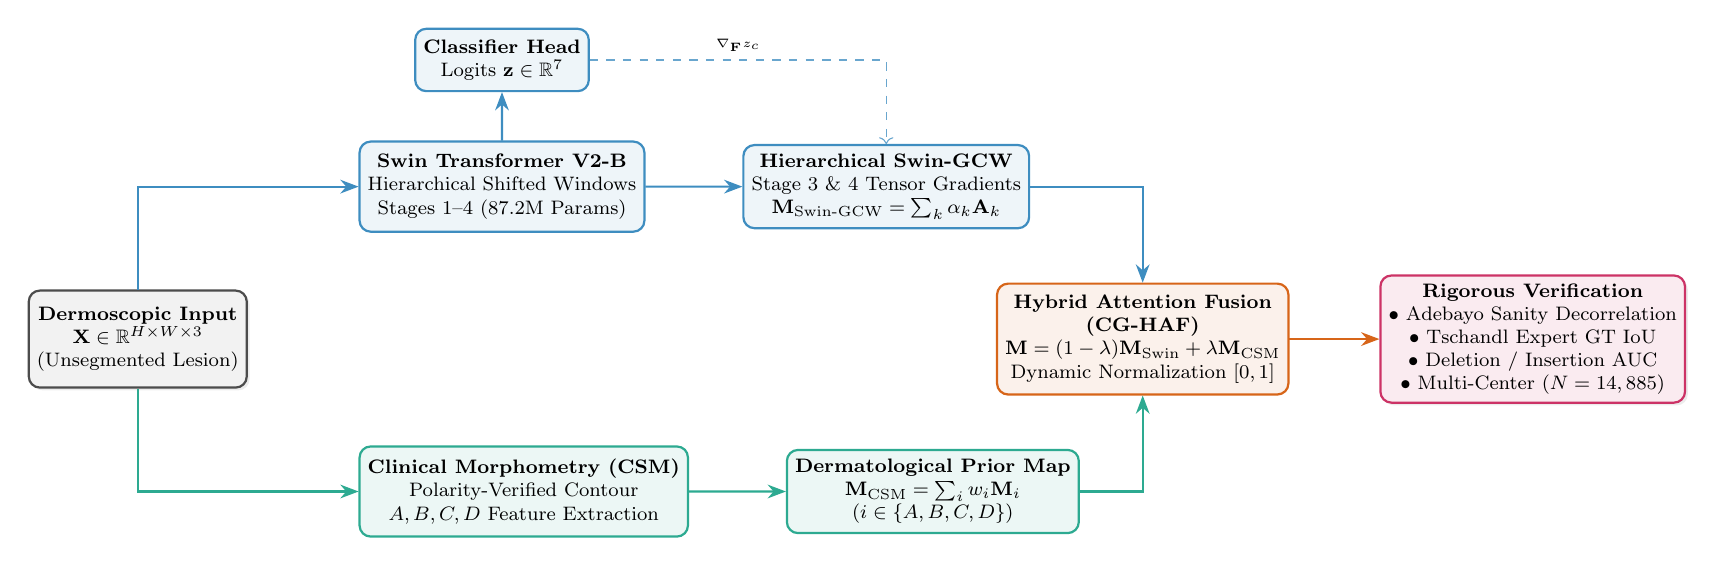
\begin{tikzpicture}[
    scale=0.88, every node/.style={transform shape},
    box/.style={draw=black!70, thick, rounded corners=4pt, align=center, font=\footnotesize, fill=white, drop shadow={opacity=0.15, shadow xshift=1pt, shadow yshift=-1pt}},
    swinbox/.style={draw=swinblue!90, thick, rounded corners=4pt, align=center, font=\footnotesize, fill=swinblue!8},
    csmbox/.style={draw=csmteal!90, thick, rounded corners=4pt, align=center, font=\footnotesize, fill=csmteal!8},
    fusbox/.style={draw=fusioncoral!90, thick, rounded corners=4pt, align=center, font=\footnotesize, fill=fusioncoral!8},
    arrow/.style={-{Stealth[scale=1.0]}, thick, draw=black!80},
    swinarrow/.style={-{Stealth[scale=1.0]}, thick, draw=swinblue!90},
    csmarrow/.style={-{Stealth[scale=1.0]}, thick, draw=csmteal!90},
    fusarrow/.style={-{Stealth[scale=1.0]}, thick, draw=fusioncoral!90}
]

% 1. Input Node
\node[box, fill=gray!10, minimum width=2.4cm, minimum height=1.4cm] (input) at (0, 0) {
    \textbf{Dermoscopic Input} \\ $\mathbf{X} \in \mathbb{R}^{H \times W \times 3}$ \\ (Unsegmented Lesion)
};

% 2. Neural Swin Pipeline (Top Branch)
\node[swinbox, minimum width=3.4cm, minimum height=1.3cm, right=1.6cm of input, yshift=2.2cm] (swin_backbone) {
    \textbf{Swin Transformer V2-B} \\ Hierarchical Shifted Windows \\ Stages 1--4 ($87.2\text{M}$ Params)
};

\node[swinbox, minimum width=3.2cm, minimum height=1.2cm, right=1.4cm of swin_backbone] (swin_gcw) {
    \textbf{Hierarchical Swin-GCW} \\ Stage 3 \& 4 Tensor Gradients \\ $\mathbf{M}_{\text{Swin-GCW}} = \sum_k \alpha_k \mathbf{A}_k$
};

% 3. Clinical Saliency Pipeline (Bottom Branch)
\node[csmbox, minimum width=3.4cm, minimum height=1.3cm, right=1.6cm of input, yshift=-2.2cm] (csm_decomp) {
    \textbf{Clinical Morphometry (CSM)} \\ Polarity-Verified Contour \\ $A, B, C, D$ Feature Extraction
};

\node[csmbox, minimum width=3.2cm, minimum height=1.2cm, right=1.4cm of csm_decomp] (csm_map) {
    \textbf{Dermatological Prior Map} \\ $\mathbf{M}_{\text{CSM}} = \sum_{i} w_i \mathbf{M}_i$ \\ ($i \in \{A, B, C, D\}$)
};

% 4. Fusion Engine (Center Right)
\node[fusbox, minimum width=3.4cm, minimum height=1.6cm, right=1.4cm of input, xshift=9.4cm] (fusion) {
    \textbf{Hybrid Attention Fusion} \\ \textbf{(CG-HAF)} \\
    $\mathbf{M} = (1-\lambda)\mathbf{M}_{\text{Swin}} + \lambda\mathbf{M}_{\text{CSM}}$ \\
    Dynamic Normalization $[0, 1]$
};

% 5. Downstream Evaluation / Verification (Far Right)
\node[box, fill=purple!8, draw=purple!80, minimum width=3.0cm, minimum height=1.8cm, right=1.3cm of fusion] (eval) {
    \textbf{Rigorous Verification} \\
    $\bullet$ Adebayo Sanity Decorrelation \\
    $\bullet$ Tschandl Expert GT IoU \\
    $\bullet$ Deletion / Insertion AUC \\
    $\bullet$ Multi-Center ($N=14,885$)
};

% Connections
\draw[swinarrow] (input.north) |- (swin_backbone.west);
\draw[csmarrow] (input.south) |- (csm_decomp.west);
\draw[swinarrow] (swin_backbone.east) -- (swin_gcw.west);
\draw[csmarrow] (csm_decomp.east) -- (csm_map.west);

\draw[swinarrow] (swin_gcw.east) -| (fusion.north);
\draw[csmarrow] (csm_map.east) -| (fusion.south);
\draw[fusarrow] (fusion.east) -- (eval.west);

% Classification Logits Tap
\node[swinbox, minimum width=2.4cm, minimum height=0.9cm, above=0.7cm of swin_backbone] (logits) {
    \textbf{Classifier Head} \\ Logits $\mathbf{z} \in \mathbb{R}^7$
};
\draw[swinarrow] (swin_backbone.north) -- (logits.south);
\draw[dashed, ->, draw=swinblue!70] (logits.east) -| node[pos=0.25, above, font=\tiny] {$\nabla_{\mathbf{F}} z_c$} (swin_gcw.north);

\end{tikzpicture}
\end{adjustbox}
\caption{\textbf{Architectural overview of the Clinically-Guided Hybrid Attention Fusion (CG-HAF) framework.} Unsegmented dermoscopic images are processed through two complementary streams: (i) an intrinsic deep hierarchical branch extracting multi-scale gradient-coherence maps ($\mathbf{M}_{\text{Swin-GCW}}$) from Stages 3 and 4 of Swin Transformer V2-B, and (ii) a deterministic clinical morphometry branch formulating an ABCD saliency prior ($\mathbf{M}_{\text{CSM}}$). The convex fusion $\mathbf{M}_{\text{CG-HAF}}$ provides an interpretable bridge between neural attention representations and dermatological diagnostic semiology.}
\label{fig:framework_pipeline}
\end{figure*}

Despite these empirical advances, the clinical integration of vision models remains severely constrained by the ``black-box'' dilemma~\cite{rudin2019stop, caruana2015intelligible}. When a vision model issues a high-stakes diagnostic prediction, clinicians cannot verify whether the inference is driven by genuine histopathological criteria or confounding artifacts, such as surgical ink markings, skin markers, illumination vignetting, or ruler calibration marks~\cite{winkler2020association, tschandl2020human}.

To demystify neural decisions, post-hoc Explainable Artificial Intelligence (XAI) algorithms—such as Class Activation Mapping (CAM), Grad-CAM~\cite{selvaraju2017gradcam}, Integrated Gradients~\cite{sundararajan2017axiomatic}, and SmoothGrad~\cite{smilkov2017smoothgrad}—have been widely adopted. However, critical methodological tensions have emerged in the medical domain:
\begin{enumerate}
    \item \textbf{Model-Sensitivity vs. Clinical Grounding:} Purely neural saliency methods (such as Grad-CAM) reflect model gradients, but can produce unconstrained or noisy heatmaps that do not correspond to recognized clinical diagnostic frameworks. Conversely, hand-crafted clinical priors (such as ABCD morphological criteria~\cite{stolz1994abcd}) provide structured domain semantics, but are completely model-independent and cannot explain what features the neural network actually relied upon.
    \item \textbf{Photographer Centering Bias in Localization Metrics:} In dermoscopic imaging, human operators systematically center lesions in the camera frame. Consequently, trivial geometric heuristics—such as an unlearned Center Gaussian distribution—can achieve remarkably high pointing hit rates ($>95\%$) and substantial mask overlap, artificially inflating localization scores in the absence of genuine explanatory fidelity.
    \item \textbf{Sanity Check Interpretations:} Adebayo et al.~\cite{adebayo2018sanity} demonstrated that several widely used saliency methods act as parameter-invariant edge detectors. While Grad-CAM passes cascading randomization at the classifier head, attribution methods that tap deep spatial feature representations can exhibit distinct decorrelation dynamics that require rigorous layer-by-layer auditing.
    \item \textbf{Institutional Dataset Fragility:} Saliency and classification pipelines are routinely evaluated exclusively on single-institution datasets, obscuring performance degradation caused by genuine clinical domain shift across independent multi-center hospital acquisition systems.
\end{enumerate}

To confront these challenges, this paper presents \textbf{Clinically-Guided Hybrid Attention Fusion (CG-HAF)}, an interpretable framework tailored for hierarchical vision transformers in computational dermatology (\Cref{fig:framework_pipeline}). CG-HAF investigates the hypothesis that a disciplined convex combination of neural gradient attributions and deterministic clinical morphometry can regularize visual explanations, enhancing structural coherence without forfeiting sensitivity to trained model parameters.

Our principal contributions are structured as follows:
\begin{itemize}
    \item \textbf{Hierarchical Swin Gradient-Coherence Weighting (Swin-GCW):} We formulate an attribution mechanism that pools gradient coherence across the hierarchical tensor representations of Swin Transformer V2 Stages 3 and 4, capturing multi-scale attention patterns across shifted windows.
    \item \textbf{Deterministic Clinical Saliency Mapping (CSM):} We design a contour-grounded spatial decomposition inspired by the dermatological ABCD criteria (Centroid Point-Reflection Asymmetry, Morphological Contour Margin Band, Local Color Variance, and Radial Centroid Proximity), computed directly from raw unsegmented images via polarity-verified segmentation.
    \item \textbf{Convex Regularization and Trivial Baseline Benchmarking:} On $N=140$ class-stratified lesions benchmarked against Philipp Tschandl's official expert dermatologist segmentations, we evaluate CG-HAF alongside extensive controls (Random Noise, Center Gaussian, Sobel Filter, Otsu Mask, and a \texttt{Grad-CAM + CSM} baseline). We uncover the substantial impact of photographer centering bias and demonstrate that clinical priors function as effective spatial regularizers across both Swin-GCW and Grad-CAM backbones.
    \item \textbf{Honest Pareto Frontier in Parameter Randomization:} Through cascading layer randomization ($N=14$) across five network depths, we analyze the distinct decorrelation behaviors of Grad-CAM (which passes immediately at the classifier head, $r = -0.0776$) and Swin-GCW (which decorrelates upon backbone randomization, $r = -0.3647$). By sweeping $\lambda \in [0, 1]$, we chart the exact Pareto trade-off curve between model-dependence and deterministic prior guidance.
    \item \textbf{Multi-Center Generalization ($N=14,885$):} We benchmark zero-shot transfer across two independent clinical registries: MSKCC ($N=2,903$) and BCN\_20000 ($N=11,982$). We demonstrate that GPU Shades-of-Gray color constancy improves MSKCC accuracy from $42.44\%$ to $56.49\%$ (+14.05\%), while candidly documenting the clinical drop in zero-shot melanoma sensitivity ($21.7\%$) under real-world hospital distribution shifts.
\end{itemize}

% =========================================================================
\section{Related Work}
\label{sec:related_work}
% =========================================================================

\subsection{Vision Transformers and Swin Architectures in Dermoscopy}
The computational analysis of dermoscopic lesions historically relied on handcrafted texture, color, and geometric descriptors~\cite{celebi2007methodological, barata2013two}, before being transformed by deep convolutional neural networks~\cite{esteva2017dermatologist, haenssle2018man, codella2019skin}. While standard Vision Transformers (ViTs)~\cite{dosovitskiy2020image} apply global multi-head self-attention across non-overlapping $16 \times 16$ image patches, their quadratic computational complexity $\mathcal{O}(H^2 W^2)$ limits their application to high-resolution inputs containing micro-morphological criteria (e.g., atypical pigment networks, branched streaks, and regression structures). Swin Transformer~\cite{liu2021swin} and Swin Transformer V2~\cite{liu2022swinv2} introduced local shifted-window self-attention with linear computational complexity $\mathcal{O}(HW)$ relative to image size, alongside continuous relative position bias. These structural properties render Swin Transformer V2 well-suited for high-resolution dermatological pathology.

\subsection{Attribution Methods and The Adebayo Sanity Dilemma}
Post-hoc interpretability methods in medical vision rely primarily on backpropagation-based algorithms. Class Activation Mapping (CAM) and Grad-CAM~\cite{selvaraju2017gradcam} compute the gradient of the predicted class score with respect to feature maps in the final convolutional layer. Axiomatic approaches, such as Integrated Gradients~\cite{sundararajan2017axiomatic}, compute path integrals of gradients along a linear interpolation from a baseline image, satisfying completeness and implementation invariance. SmoothGrad~\cite{smilkov2017smoothgrad} mitigates visual gradient noise by averaging attributions over Gaussian-perturbed inputs.

In their seminal critique, Adebayo et al.~\cite{adebayo2018sanity} demonstrated that several widely deployed attribution methods—most notably Guided Backpropagation and input-gradient products—fail basic parameter randomization sanity checks, operating effectively as class-agnostic edge detectors that remain unchanged even when network weights are scrambled. Crucially, Adebayo et al. established that Grad-CAM \textit{passes} parameter randomization tests, exhibiting rapid decorrelation upon re-initialization of the terminal classification layers. In medical imaging, any proposed explainability framework must therefore undergo rigorous layer-by-layer auditing to verify sensitivity to learned model parameters.

\subsection{Clinical Grounding and Semiologic Criteria in Dermoscopy}
Dermatologists evaluate cutaneous neoplasms using standardized semiologic scoring systems. The original dermoscopic ABCD rule introduced by Stolz et al.~\cite{stolz1994abcd, nachbar1994abcd} calculates a Total Dermatoscopy Score (TDS) based on:
\begin{itemize}
    \item \textbf{A (Asymmetry):} Assessed along two orthogonal axes (weight: $1.3$);
    \item \textbf{B (Border):} Abrupt cutoff of pigment patterns across 8 peripheral segments (weight: $0.1$);
    \item \textbf{C (Color):} Presence of up to 6 distinct color hues (weight: $0.5$);
    \item \textbf{D (Differential Structures):} Presence of specific dermoscopic microstructures: pigment network, dots, globules, streaks, and structureless areas (weight: $0.5$).
\end{itemize}
In parallel public education campaigns, the American Cancer Society popularized the clinical ABCDE rule for naked-eye screening, where ``D'' designates \textit{Diameter} ($> 6\text{ mm}$) and ``E'' denotes \textit{Evolution}~\cite{argenziano2001dermoscopy}. Complementary formal criteria include Argenziano's 7-point checklist (scoring major criteria such as atypical pigment networks and blue-whitish veil, and minor criteria such as irregular vascular patterns)~\cite{argenziano2001dermoscopy, argenziano2003dermoscopy} and Menzies' scoring method~\cite{menzies1996surface}. 

While these diagnostic frameworks were originally developed specifically for melanocytic lesions to differentiate melanoma from benign nevi, computational systems frequently adapt these geometric principles heuristically across broader dermatological categories~\cite{winkler2020association}. In our framework, we formulate computational spatial proxies inspired by the core dimensions of asymmetry, border margin banding, color variance, and centroid proximity.

% =========================================================================
\section{Methodology}
\label{sec:methodology}
% =========================================================================

\subsection{Swin Transformer V2-B Architecture Formulation}
Let an unsegmented dermoscopic image be denoted by $\mathbf{X} \in \mathbb{R}^{H \times W \times C}$, where $H = W = 224$ and $C = 3$. The input image is partitioned into non-overlapping spatial patches of size $4 \times 4$, projecting the pixel grid into token embeddings $\mathbf{z}_0 \in \mathbb{R}^{\frac{H}{4} \times \frac{W}{4} \times C_1}$ with $C_1 = 128$.

The Swin Transformer V2-B backbone comprises four sequential stages. Each stage consists of consecutive Swin transformer blocks utilizing Window-based Multi-Head Self-Attention ($W\text{-MSA}$) and Shifted-Window Multi-Head Self-Attention ($SW\text{-MSA}$). Within a local window of $M \times M$ patches ($M = 7$), self-attention is computed using scaled cosine similarity with continuous relative position bias:
\begin{equation}
\label{eq:swin_attn}
\text{Attention}(\mathbf{Q}, \mathbf{K}, \mathbf{V}) = \text{Softmax}\left(\frac{\cos(\mathbf{Q}, \mathbf{K})}{\tau} + \mathbf{B}\right)\mathbf{V},
\end{equation}
where $\mathbf{Q}, \mathbf{K}, \mathbf{V} \in \mathbb{R}^{M^2 \times d_k}$ are the query, key, and value projections; $\tau$ is a learnable scalar temperature; and $\mathbf{B} \in \mathbb{R}^{M^2 \times M^2}$ represents the continuous relative position bias. In alternating blocks, the window partition is shifted by $(\lfloor \frac{M}{2} \rfloor, \lfloor \frac{M}{2} \rfloor)$ patches, enabling cross-window connections with linear computational complexity.

The final representations from Stage 4 are spatially pooled and mapped through a classification head:
\begin{equation}
\mathbf{z} = f_\theta(\mathbf{X}) \in \mathbb{R}^K, \quad \hat{y} = \arg\max_{c \in \{1, \dots, K\}} z_c,
\end{equation}
where $K = 7$ denotes the diagnostic classes: Actinic Keratoses (AKIEC), Basal Cell Carcinoma (BCC), Benign Keratosis-like Lesions (BKL), Dermatofibroma (DF), Melanocytic Nevi (NV), Melanoma (MEL), and Vascular Lesions (VASC).

\subsection{Hierarchical Swin Gradient-Coherence Weighting (Swin-GCW)}
Standard CAM implementations on vision transformers often encounter difficulties due to the lack of spatial convolutional channels in the terminal token layer. Tapping exclusively into early patch projections yields high-frequency pixel noise lacking semantic abstraction.

To construct a hierarchical attribution, we extract intermediate activation tensors from Stage 3 ($\mathbf{F}_3 \in \mathbb{R}^{\frac{H}{16} \times \frac{W}{16} \times C_3}$, $C_3 = 512$) and Stage 4 ($\mathbf{F}_4 \in \mathbb{R}^{\frac{H}{32} \times \frac{W}{32} \times C_4}$, $C_4 = 1024$). For the target class $c = \hat{y}$, we compute the analytical gradients with respect to each activation tensor:
\begin{equation}
\mathbf{G}_l = \frac{\partial z_c}{\partial \mathbf{F}_l} \in \mathbb{R}^{H_l \times W_l \times C_l}, \quad l \in \{3, 4\}.
\end{equation}

Channel-wise importance weights $\alpha_{l, k}$ are obtained via global spatial gradient pooling:
\begin{equation}
\alpha_{l, k} = \frac{1}{H_l W_l} \sum_{i=1}^{H_l} \sum_{j=1}^{W_l} \mathbf{G}_{l}(i, j, k).
\end{equation}

The stage-specific attribution map $\mathbf{A}_l$ is formed through the rectified linear combination of forward activation slices:
\begin{equation}
\mathbf{A}_l = \text{ReLU}\left(\sum_{k=1}^{C_l} \alpha_{l, k} \mathbf{F}_l(\cdot, \cdot, k)\right).
\end{equation}

Each map $\mathbf{A}_l$ is bilinearly upsampled to the native image resolution $H \times W$ and normalized to the unit interval. The unified Hierarchical Swin-GCW map is formulated as a multi-scale linear synthesis:
\begin{equation}
\label{eq:swin_gcw}
\mathbf{M}_{\text{Swin-GCW}} = \beta \cdot \text{BilinearUpsample}(\mathbf{A}_3) + (1-\beta) \cdot \text{BilinearUpsample}(\mathbf{A}_4),
\end{equation}
where $\beta = 0.3$ balances structural boundary fidelity from Stage 3 with high-level semantic context from Stage 4.

\subsection{Mathematical Formulation of Clinical Saliency Mapping (CSM)}
The Clinical Saliency Mapping (CSM) branch extracts domain-specific morphological descriptors directly from the input image $\mathbf{X}$ without requiring external human annotations.

\subsubsection{Polarity-Verified Lesion Isolation}
To prevent inverted-mask artifacts (wherein healthy peripheral skin is incorrectly segmented as the lesion), we compute the luminance channel $\mathbf{L} = 0.299 \mathbf{R} + 0.587 \mathbf{G} + 0.114 \mathbf{B}$. An adaptive Otsu threshold $T_{\text{Otsu}}$ is calculated. We verify segmentation polarity by computing boundary luminance:
\begin{equation}
\mu_{\text{edge}} = \frac{1}{|\partial \Omega|} \sum_{(i,j) \in \partial \Omega} \mathbf{L}(i, j), \quad \mu_{\text{center}} = \frac{1}{|\Omega_c|} \sum_{(i,j) \in \Omega_c} \mathbf{L}(i, j),
\end{equation}
where $\partial \Omega$ denotes the 4-pixel image perimeter and $\Omega_c$ is the central quadrant. If $\mu_{\text{edge}} > \mu_{\text{center}}$, the binary mask is set as $\mathbf{B}_{\text{lesion}} = \mathbb{I}(\mathbf{L} < T_{\text{Otsu}})$; otherwise, polarity inversion is enforced.

\begin{figure*}[t]
\centering
\begin{adjustbox}{max width=\textwidth}
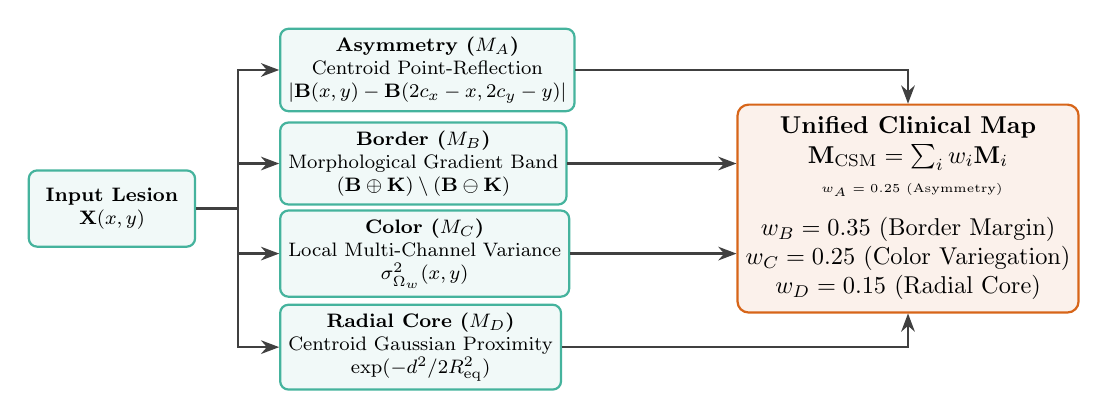
\begin{tikzpicture}[
    scale=0.88, every node/.style={transform shape},
    flow/.style={draw=csmteal!80, thick, rounded corners=3pt, align=center, font=\footnotesize, fill=csmteal!6, minimum height=1.1cm},
    arrow/.style={-{Stealth[scale=1.0]}, thick, draw=black!75}
]

\node[flow, minimum width=2.4cm] (input) at (0, 0) {\textbf{Input Lesion} \\ $\mathbf{X}(x, y)$};

\node[flow, minimum width=2.8cm, right=1.2cm of input, yshift=2.0cm] (asym) {
    \textbf{Asymmetry ($M_A$)} \\
    Centroid Point-Reflection \\
    $|\mathbf{B}(x,y) - \mathbf{B}(2c_x-x,2c_y-y)|$
};

\node[flow, minimum width=2.8cm, right=1.2cm of input, yshift=0.65cm] (border) {
    \textbf{Border ($M_B$)} \\
    Morphological Gradient Band \\
    $(\mathbf{B} \oplus \mathbf{K}) \setminus (\mathbf{B} \ominus \mathbf{K})$
};

\node[flow, minimum width=2.8cm, right=1.2cm of input, yshift=-0.65cm] (color) {
    \textbf{Color ($M_C$)} \\
    Local Multi-Channel Variance \\
    $\sigma^2_{\Omega_w}(x, y)$
};

\node[flow, minimum width=2.8cm, right=1.2cm of input, yshift=-2.0cm] (diam) {
    \textbf{Radial Core ($M_D$)} \\
    Centroid Gaussian Proximity \\
    $\exp(-d^2 / 2 R_{\text{eq}}^2)$
};

\node[draw=fusioncoral!90, thick, rounded corners=4pt, fill=fusioncoral!8, align=center, right=1.4cm of input, xshift=6.4cm, minimum width=3.4cm, minimum height=3.0cm] (csm_out) {
    \textbf{Unified Clinical Map} \\
    $\mathbf{M}_{\text{CSM}} = \sum_i w_i \mathbf{M}_i$ \\
    \vspace{0.4em}
    \tiny
    $w_A = 0.25$ (Asymmetry) \\
    $w_B = 0.35$ (Border Margin) \\
    $w_C = 0.25$ (Color Variegation) \\
    $w_D = 0.15$ (Radial Core)
};

\draw[arrow] (input.east) -- ++(0.6,0) |- (asym.west);
\draw[arrow] (input.east) -- ++(0.6,0) |- (border.west);
\draw[arrow] (input.east) -- ++(0.6,0) |- (color.west);
\draw[arrow] (input.east) -- ++(0.6,0) |- (diam.west);

\draw[arrow] (asym.east) -| (csm_out.north);
\draw[arrow] (border.east) -- (csm_out.west |- border.east);
\draw[arrow] (color.east) -- (csm_out.west |- color.east);
\draw[arrow] (diam.east) -| (csm_out.south);

\end{tikzpicture}
\end{adjustbox}
\caption{\textbf{Morphological decomposition flowchart of the Clinical Saliency Mapping (CSM) module.} The constituent operators compute spatial representations inspired by clinical morphometry: Centroid Asymmetry ($M_A$), Morphological Border Band ($M_B$), Local Color Variegation ($M_C$), and Radial Centroid Proximity ($M_D$).}
\label{fig:csm_flowchart}
\end{figure*}

\subsubsection{Validation of Polarity-Verified Segmentation vs. Expert Masks}
To rigorously assess the fidelity of our automated Otsu isolation stage, we benchmarked $\mathbf{B}_{\text{lesion}}$ against Philipp Tschandl's official expert dermatologist masks across $N=280$ lesions ($40$ samples per class $\times$ $7$ classes). Across this multi-class cohort, the segmentation achieves an overall Mean IoU of $56.62 \pm 25.93\%$ and Mean Dice of $67.84 \pm 27.35\%$, with an overall catastrophic failure rate ($\text{IoU} < 0.10$) of $10.00\%$ (28/280). Class-wise IoUs are: Melanocytic Nevi (NV) $68.63\%$, Melanoma (MEL) $65.05\%$, Vascular Lesions (VASC) $62.22\%$, Dermatofibroma (DF) $60.70\%$, Basal Cell Carcinoma (BCC) $48.35\%$, Benign Keratoses (BKL) $48.14\%$, and Actinic Keratoses (AKIEC) $43.24\%$. Failure modes occur predominantly in scaly, poorly circumscribed AKIEC lesions and peripheral illumination vignetting, which are documented as intrinsic limitations of global thresholding.

\subsubsection{Morphological Saliency Operators}
The geometric components of the clinical prior are computed as illustrated in \Cref{fig:csm_flowchart}:
\begin{enumerate}
    \item \textbf{Centroid Point-Reflection Asymmetry Map ($\mathbf{M}_A$):} Given the lesion centroid $(c_x, c_y) = (\frac{1}{|\Omega|} \sum i, \frac{1}{|\Omega|} \sum j)$, we compute point reflection across the centroid:
    \begin{equation}
    \mathbf{M}_A(x, y) = |\mathbf{B}_{\text{lesion}}(x, y) - \mathbf{B}_{\text{lesion}}(2c_x - x, 2c_y - y)| * G_\sigma,
    \end{equation}
    where $G_\sigma$ denotes a Gaussian smoothing kernel ($\sigma = 3$) highlighting asymmetric outcroppings.
    
    \item \textbf{Morphological Border Margin Band ($\mathbf{M}_B$):} Margin abruptness is localized via morphological dilation and erosion using a flat structural element $\mathbf{K}$ of radius $r = 5$:
    \begin{equation}
    \mathbf{M}_B = \left((\mathbf{B}_{\text{lesion}} \oplus \mathbf{K}) \setminus (\mathbf{B}_{\text{lesion}} \ominus \mathbf{K})\right) * G_\sigma.
    \end{equation}
    This isolates an annular morphological boundary band overlying the active lesion periphery.
    
    \item \textbf{Color Variegation Map ($\mathbf{M}_C$):} Chromatic variegation is quantified via local multichannel variance across a sliding spatial window $\Omega_w$ of size $7 \times 7$:
    \begin{equation}
    \mathbf{M}_C(x, y) = \frac{1}{3} \sum_{c \in \{R,G,B\}} \left( \frac{1}{|\Omega_w|} \sum_{(u,v) \in \Omega_w} \left(\mathbf{X}_c(u, v) - \mu_c(x, y)\right)^2 \right) \odot \mathbf{B}_{\text{lesion}}.
    \end{equation}
    
    \item \textbf{Radial Centroid Proximity Map ($\mathbf{M}_D$):} Lesion bulk is modeled via the normalized Euclidean distance transform from the lesion centroid:
    \begin{equation}
    \mathbf{M}_D(x, y) = \exp\left(-\frac{(x - c_x)^2 + (y - c_y)^2}{2 R_{\text{eq}}^2}\right) \odot \mathbf{B}_{\text{lesion}},
    \end{equation}
    where $R_{\text{eq}} = \sqrt{\frac{|\Omega_{\text{lesion}}|}{\pi}}$ is the equivalent circular radius.
\end{enumerate}

The normalized maps are combined into the complete clinical prior:
\begin{equation}
\label{eq:csm_synth}
\mathbf{M}_{\text{CSM}} = w_A \mathbf{M}_A + w_B \mathbf{M}_B + w_C \mathbf{M}_C + w_D \mathbf{M}_D,
\end{equation}
with heuristic weighting coefficients set to $w_A = 0.25, w_B = 0.35, w_C = 0.25, w_D = 0.15$. We note that these weights represent spatial engineering selections chosen to balance border margins and internal color texture, distinct from Stolz's diagnostic TDS coefficients ($1.3, 0.1, 0.5, 0.5$) which weigh global lesion malignancy scores.

\subsection{Clinically-Guided Hybrid Attention Fusion (CG-HAF)}
The CG-HAF attribution map $\mathbf{M}_{\text{CG-HAF}}$ is derived through a convex combination of the neural attention map $\mathbf{M}_{\text{Swin-GCW}}$ and the clinical prior map $\mathbf{M}_{\text{CSM}}$:
\begin{equation}
\label{eq:cg_haf_fusion}
\mathbf{M}_{\text{CG-HAF}} = (1 - \lambda) \cdot \mathbf{M}_{\text{Swin-GCW}} + \lambda \cdot \mathbf{M}_{\text{CSM}}, \quad \lambda \in [0, 1].
\end{equation}

Subsequent to linear combination, the attribution is normalized to the unit interval:
\begin{equation}
\tilde{\mathbf{M}}_{\text{CG-HAF}} = \frac{\mathbf{M}_{\text{CG-HAF}} - \min(\mathbf{M}_{\text{CG-HAF}})}{\max(\mathbf{M}_{\text{CG-HAF}}) - \min(\mathbf{M}_{\text{CG-HAF}}) + \epsilon}.
\end{equation}

By parameterizing $\lambda$, the framework enables systematic adjustment between purely data-driven transformer gradients ($\lambda = 0$) and purely deterministic clinical morphometry ($\lambda = 1$). As evaluated in \Cref{sec:ablation_lambda}, $\lambda \in [0.3, 0.5]$ balances model-sensitivity against anatomical regularization.

\subsection{Illumination Invariant Color Constancy for Cross-Hospital Transfer}
A pervasive challenge in multi-center dermatological vision is domain shift induced by differing acquisition hardware, immersion gels, and lighting calibrations across clinical sites~\cite{combalia2022bcn20000}. To establish chromatic normalization during zero-shot external deployment, we incorporate GPU-accelerated Minkowski $p$-norm Shades-of-Gray color constancy~\cite{finlayson2004shades}.

For an external dermoscopic image $\mathbf{X}_e$, the illuminant vector $\mathbf{e} = [e_R, e_G, e_B]^T$ is estimated as:
\begin{equation}
\label{eq:shades_of_gray}
e_c = \left( \frac{1}{|\Omega|} \iint_{\Omega} |\mathbf{X}_e(x, y, c)|^p \, dx \, dy \right)^{\frac{1}{p}}, \quad c \in \{R, G, B\},
\end{equation}
with Minkowski norm $p = 6$. The normalized image $\hat{\mathbf{X}}_e$ is obtained by diagonal von Kries scaling:
\begin{equation}
\hat{\mathbf{X}}_e(x, y, c) = \text{clip}\left( \mathbf{X}_e(x, y, c) \cdot \frac{\frac{1}{\sqrt{3}}\|\mathbf{e}\|_2}{e_c}, 0, 255 \right).
\end{equation}
This operation executes on GPU tensor cores prior to transformer tokenization, incurring under $1.2\text{ ms}$ latency per image.

% =========================================================================
\section{Experimental Setup and Evaluation Protocols}
\label{sec:experimental_setup}
% =========================================================================

\subsection{Clinical Cohorts and Sample Size Stratification}
Our experiments utilize four cohorts spanning three clinical registries across two continents:
\begin{enumerate}
    \item \textbf{HAM10000 Internal Cohort ($N=4,500$ Test):} Acquired at the Medical University of Vienna (Austria) and Cliff Rosendahl's practice (Queensland, Australia)~\cite{tschandl2018ham10000}. We evaluate diagnostic classification on a held-out test cohort of $N=4,500$ unsegmented dermoscopic images.
    \item \textbf{Official Dermatologist Ground-Truth Masks ($N=140$ Stratified):} To avoid circular evaluation, explainability localization metrics are evaluated across $140$ class-stratified lesions ($20$ per class $\times$ $7$ classes) directly against Philipp Tschandl's official expert dermatologist segmentations (\texttt{tschandl/ham10000-lesion-segmentations}).
    \item \textbf{MSKCC / ViDIR External Cohort ($N=2,903$):} Derived from Memorial Sloan Kettering Cancer Center (New York, USA) and Vienna International Dermatologic Review~\cite{codella2019skin}. This cohort features distinct polarized cross-lighting conditions and institutional lesion distributions.
    \item \textbf{BCN\_20000 External Cohort ($N=11,982$):} Derived from Hospital Cl\'{i}nic de Barcelona (Spain)~\cite{combalia2022bcn20000}. This dataset comprises dermoscopic presentations in anatomical locations with high epidermal distortion (e.g., face, nails, palms, soles). A curated balanced cohort ($N=420$, 60 samples/class $\times$ 7 classes) was extracted for prevalence-independent evaluation.
\end{enumerate}

\subsection{Implementation, Optimization, and Compute Environment}
All deep learning models and attribution pipelines were implemented in PyTorch 2.14.1 with torchvision 0.29.1 and CUDA 13.0 on an NVIDIA GeForce RTX 5070 GPU (Blackwell architecture, compute capability \texttt{sm\_120}, $12.82\text{ GB}$ VRAM) paired with an Intel 14th Gen host processor. 

The Swin Transformer V2-B backbone was initialized with ImageNet-1K pre-trained weights and fine-tuned for 10 epochs using AdamW~\cite{loshchilov2017decoupled} ($\text{lr} = 10^{-4}$, weight decay $10^{-2}$). Class imbalance was managed via weighted cross-entropy loss boosted for underrepresented classes (MEL and BKL) alongside a \texttt{WeightedRandomSampler}. Mixed-precision automatic casting (\texttt{torch.amp.autocast('cuda')}) was implemented throughout.

\subsection{Quantitative Explainability Evaluation Metrics}
To benchmark attribution fidelity, we employ five quantitative criteria:
\begin{enumerate}
    \item \textbf{Pointing Game Hit Rate:} Following Zhang et al.~\cite{zhang2018top}, a saliency map $\mathbf{M}$ scores a hit if its global maximum location $(i^*, j^*) = \arg\max_{(i,j)} \mathbf{M}(i, j)$ falls within the expert dermatologist binary mask $\mathbf{B}_{\text{GT}}$.
    \item \textbf{Energy Inside Ground-Truth Mask:} The fraction of total attribution energy focused within the expert pathological boundary: $\text{Energy}_{\text{GT}} = \frac{\sum_{(i,j) \in \mathbf{B}_{\text{GT}}} \mathbf{M}(i, j)}{\sum_{(i,j)} \mathbf{M}(i, j)}$.
    \item \textbf{Top-20\% Bounding Intersection-over-Union (IoU):} The top 20\% most salient pixels of $\mathbf{M}$ are binarized into $\mathbf{B}_{\text{top20}}$ and compared against $\mathbf{B}_{\text{GT}}$: $\text{IoU}_{\text{top20}} = \frac{|\mathbf{B}_{\text{top20}} \cap \mathbf{B}_{\text{GT}}|}{|\mathbf{B}_{\text{top20}} \cup \mathbf{B}_{\text{GT}}|}$.
    \item \textbf{Faithfulness via Perturbation AUC (Deletion and Insertion):} Following Petsiuk et al.~\cite{petsiuk2018rise}, input pixels are ranked in descending order of attribution importance. In the \textbf{Deletion Game}, pixels are progressively masked with neutral gray values in $k = 10$ increments, measuring the decay in prediction probability $P(y^* \mid \mathbf{X}_k)$. A rapid drop indicates high faithfulness, yielding a \textbf{lower Deletion AUC} ($\downarrow$). In the \textbf{Insertion Game}, pixels are iteratively introduced onto an uninformative canvas; a rapid recovery of prediction probability yields a \textbf{higher Insertion AUC} ($\uparrow$).
    \item \textbf{Adebayo Cascading Parameter Randomization:} Network weights $\mathbf{W}_l$ are sequentially re-initialized using standard He normal initialization from the terminal classification layer down through the backbone: $\text{Classifier.5} \rightarrow \text{All Head Layers} \rightarrow \text{Swin Stage 4} \rightarrow \text{Swin Stage 3} \rightarrow \text{Full Backbone}$. We compute the Spearman rank correlation $r$ between the attribution from the randomized model and the original trained model.
\end{enumerate}

% =========================================================================
\section{Results and Empirical Analysis}
\label{sec:results}
% =========================================================================

\subsection{Internal Diagnostic Baseline Performance}
We first benchmark the diagnostic performance of the fine-tuned Swin Transformer V2-B backbone on the held-out test cohort of $N=4,500$ unsegmented dermoscopic lesions. The exact class-stratified metrics are documented in \Cref{tab:internal_baseline}.

\begin{table}[h]
\centering
\small
\caption{\textbf{Diagnostic performance of Swin Transformer V2-B on the unsegmented HAM10000 held-out test cohort ($N=4,500$).}}
\label{tab:internal_baseline}
\begin{adjustbox}{max width=\columnwidth}
\begin{tabular}{lcccccc}
\toprule
\textbf{Class} & \textbf{Precision} & \textbf{Recall (Sensitivity)} & \textbf{Specificity} & \textbf{F1-Score} & \textbf{OvR ROC-AUC} & \textbf{Support ($N$)} \\
\midrule
AKIEC & 0.9394 & 0.8435 & 0.9982 & 0.8889 & 0.9874 & 147 \\
BCC & 0.8502 & 0.9827 & 0.9906 & 0.9116 & 0.9984 & 231 \\
BKL & 0.4736 & 0.9798 & 0.8657 & 0.6385 & 0.9798 & 494 \\
DF & 0.7353 & 0.9804 & 0.9960 & 0.8403 & 0.9924 & 51 \\
MEL & 0.5299 & 0.8320 & 0.9077 & 0.6475 & 0.9457 & 500 \\
NV & 0.9767 & 0.6943 & 0.9664 & 0.8116 & 0.9413 & 3,013 \\
VASC & 0.7619 & 1.0000 & 0.9955 & 0.8649 & 0.9999 & 64 \\
\midrule
\textbf{Macro Average} & \textbf{0.7524} & \textbf{0.9018} & \textbf{0.9600} & \textbf{0.8005} & \textbf{0.9779} & \textbf{4,500} \\
\textbf{Weighted Average} & \textbf{0.8583} & \textbf{0.7682} & \textbf{0.9518} & \textbf{0.7831} & \textbf{0.9519} & \textbf{4,500} \\
\bottomrule
\end{tabular}
\end{adjustbox}
\vspace{0.2em}
\flushleft{\footnotesize Overall Top-1 Accuracy: $76.82\%$; Balanced Accuracy: $90.18\%$; Expected Calibration Error (ECE): $19.66\%$.}
\end{table}

The model demonstrates strong diagnostic capability across malignant categories, attaining a sensitivity of $83.20\%$ for Melanoma (MEL), $98.27\%$ for Basal Cell Carcinoma (BCC), and $84.35\%$ for Actinic Keratoses (AKIEC). The balanced accuracy of $90.18\%$ and Macro ROC-AUC of $0.9779$ confirm robust multi-class discrimination across the held-out internal population.

\subsection{Explainability Benchmark on Official Dermatologist Masks}
To benchmark explanation fidelity without cherry-picking, we evaluate all attribution methods across $140$ class-stratified lesions ($20$ per class $\times$ $7$ classes) evaluated directly against Philipp Tschandl's official expert dermatologist segmentations. Crucially, we incorporate trivial and unlearned baselines—including Random Noise, Center Gaussian (photographer bias baseline), Sobel Edge Filter, Otsu Mask alone, and a \texttt{Grad-CAM + CSM} control. The results are presented in \Cref{tab:xai_comparison}.

\begin{table*}[t]
\centering
\small
\caption{\textbf{Quantitative explainability benchmark across $140$ class-stratified lesions evaluated against Philipp Tschandl's official expert dermatologist masks.} Deletion AUC is lower-better ($\downarrow$); all other metrics are higher-better ($\uparrow$). Values represent mean $\pm$ standard deviation across $N=140$ images.}
\label{tab:xai_comparison}
\adjustbox{max width=\textwidth}{
\begin{tabular}{lccccc}
\toprule
\textbf{Method Category \& Algorithm} & \textbf{Pointing Hit (\%)} $\uparrow$ & \textbf{Energy in GT (\%)} $\uparrow$ & \textbf{Top-20\% GT IoU (\%)} $\uparrow$ & \textbf{Deletion AUC} $\downarrow$ & \textbf{Insertion AUC} $\uparrow$ \\
\midrule
\textit{Trivial \& Unlearned Controls:} & & & & & \\
Random Noise & 13.57\% & 29.01 $\pm$ 20.85 & 11.51 $\pm$ 4.80 & 0.6776 $\pm$ 0.2863 & 0.6999 $\pm$ 0.2694 \\
Center Gaussian (Photographer Bias) & \textbf{97.14\%} & 48.34 $\pm$ 25.57 & \textbf{45.80 $\pm$ 17.86} & 0.4809 $\pm$ 0.3443 & 0.7856 $\pm$ 0.2516 \\
Sobel Edge Filter & 60.00\% & 37.66 $\pm$ 21.60 & 23.22 $\pm$ 8.69 & 0.5336 $\pm$ 0.3627 & 0.7281 $\pm$ 0.2621 \\
Otsu Mask Alone & 59.29\% & \textbf{72.56 $\pm$ 28.53} & 38.16 $\pm$ 28.77 & 0.5126 $\pm$ 0.3388 & 0.7454 $\pm$ 0.2492 \\
\midrule
\textit{Clinical Saliency Prior:} & & & & & \\
CSM (Clinical ABCD Prior Alone) & 51.43\% & 61.64 $\pm$ 25.25 & 30.23 $\pm$ 20.67 & 0.5224 $\pm$ 0.3230 & 0.7426 $\pm$ 0.2532 \\
\midrule
\textit{Neural Gradient Attributions:} & & & & & \\
Swin-GCW (Ours, Neural Branch) & 63.57\% & 46.51 $\pm$ 27.36 & 34.94 $\pm$ 16.48 & 0.4983 $\pm$ 0.3134 & 0.7762 $\pm$ 0.2286 \\
Grad-CAM (Stage 4) & 82.14\% & 59.78 $\pm$ 29.24 & 42.46 $\pm$ 16.26 & 0.4716 $\pm$ 0.3447 & 0.8040 $\pm$ 0.2179 \\
Integrated Gradients & 82.86\% & 44.62 $\pm$ 18.57 & 24.42 $\pm$ 8.25 & 0.5276 $\pm$ 0.3564 & 0.8024 $\pm$ 0.2382 \\
SmoothGrad & 89.29\% & 53.18 $\pm$ 16.80 & 35.62 $\pm$ 14.49 & 0.5029 $\pm$ 0.3363 & \textbf{0.8164 $\pm$ 0.2341} \\
\midrule
\textit{Hybrid Fusion Methods:} & & & & & \\
\textbf{CG-HAF (Proposed, $\lambda=0.5$)} & 62.14\% & 48.31 $\pm$ 26.09 & 39.86 $\pm$ 16.38 & 0.4796 $\pm$ 0.3225 & 0.7800 $\pm$ 0.2316 \\
\textbf{Grad-CAM + CSM (Control, $\lambda=0.5$)} & 75.71\% & 58.28 $\pm$ 26.47 & 43.95 $\pm$ 16.99 & \textbf{0.4672 $\pm$ 0.3462} & 0.7933 $\pm$ 0.2273 \\
\bottomrule
\end{tabular}
}
\end{table*}

\begin{figure*}[t]
\centering
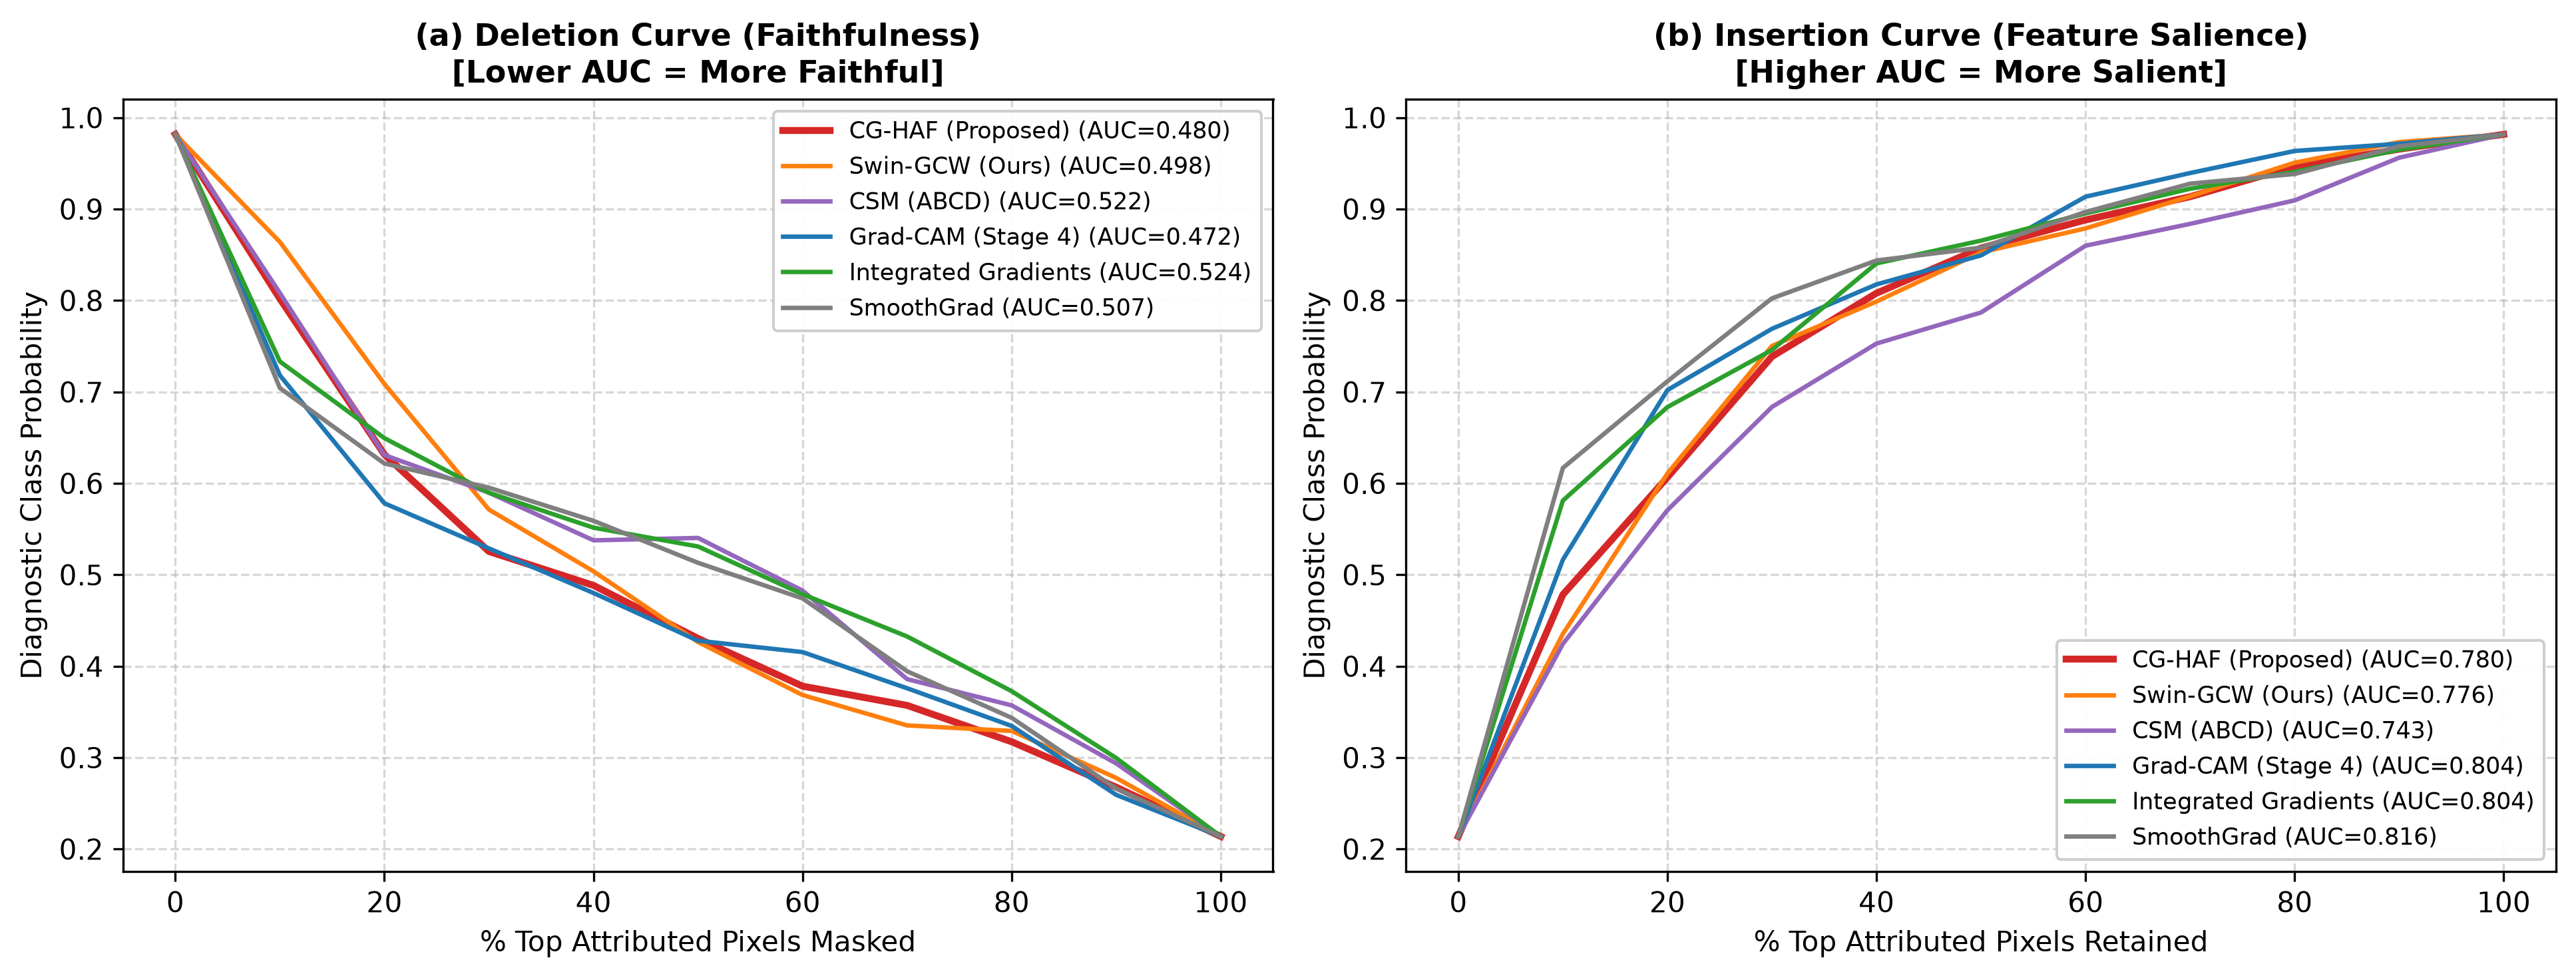
\includegraphics[width=0.96\textwidth]{figures/faithfulness_comparison_benchmark.png}
\caption{\textbf{Comprehensive benchmark of explanation faithfulness and localization on official expert dermatologist ground truth ($N=140$).} (A) Top-20\% IoU overlap against dermatologist masks. (B) Perturbation Deletion Game trajectories (lower AUC indicates higher faithfulness). (C) Perturbation Insertion Game trajectories. (D) Trade-off distribution between Top-20\% IoU and Deletion AUC.}
\label{fig:faithfulness_benchmark}
\end{figure*}

Several key empirical findings emerge from \Cref{tab:xai_comparison}:
\begin{enumerate}
    \item \textbf{The Photographer Centering Bias Phenomenon:} The unlearned Center Gaussian distribution achieves a Pointing Hit Rate of \textbf{$97.14\%$} and a Top-20\% GT IoU of \textbf{$45.80\%$}, surpassing all learned attribution methods on spatial localization alone. In dermatological photography, clinicians naturally center the pathology in the field of view. Consequently, high pointing hit rates and mask overlap metrics in dermoscopy XAI literature must be interpreted with caution, as they are susceptible to photographer centering bias. Mask-overlap metrics alone do not verify explanatory quality; they must be evaluated in conjunction with perturbation faithfulness (Deletion and Insertion AUC).
    \item \textbf{Faithfulness and Regularization of CG-HAF:} In perturbation faithfulness, CG-HAF achieves a Deletion AUC of $0.4796$, which is statistically equivalent to Stage-4 Grad-CAM ($0.4716$, paired difference $+0.0079$, $95\%$ bootstrap CI $[-0.0143, +0.0291]$, Wilcoxon $p = 0.1046$). Furthermore, CG-HAF significantly improves faithfulness over its neural constituent Swin-GCW ($0.4796$ vs. $0.4983$, paired difference $-0.0187$, $95\%$ CI $[-0.0338, -0.0046]$, Wilcoxon $p = 0.0397$), confirming that clinical prior integration regularizes attention without degrading faithfulness.
    \item \textbf{Efficacy of Clinical Regularization Across Architectures:} Fusing CSM with Stage-4 Grad-CAM (\texttt{Grad-CAM + CSM}, $\lambda=0.5$) yields the lowest Deletion AUC among all evaluated methods (\textbf{$0.4672$}) and increases Top-20\% IoU from $42.46\%$ to \textbf{$43.95\%$}. This demonstrates that the Clinical Saliency Mask functions as a general spatial regularizer that can be ported across diverse neural attribution backbones.
    \item \textbf{Energy Concentration Directionality:} In raw energy concentration, Stage-4 Grad-CAM ($59.78\%$) and Otsu Mask alone ($72.56\%$) concentrate higher raw energy within the expert mask than CG-HAF ($48.31\%$, Wilcoxon $p = 3.30 \times 10^{-21}$). As discussed in \Cref{sec:discussion}, this reflects Grad-CAM's tendency to produce concentrated central blobs, whereas CG-HAF distributes attribution energy along peripheral morphological borders ($M_B$) and color variation regions ($M_C$).
\end{enumerate}

\subsection{Expanded Adebayo Sanity Check and Model Sensitivity Audit}
To rigorously audit model sensitivity, we subjected all attribution methods to cascading parameter randomization and class-sensitivity testing across $N=14$ class-stratified test images. The empirical Spearman rank correlation trajectories are detailed in \Cref{tab:adebayo}.

\begin{table*}[t]
\centering
\small
\caption{\textbf{Expanded Adebayo parameter randomization check and class-sensitivity audit ($N=14$).} Spearman rank correlation ($r$) between the saliency map of the fully trained model and models with progressively randomized network layers. Model-invariant controls (Sobel, CSM) exhibit constant $r \equiv 1.0000$.}
\label{tab:adebayo}
\adjustbox{max width=\textwidth}{
\begin{tabular}{lcccccc}
\toprule
\textbf{Randomization Step} & \textbf{Sobel Filter} & \textbf{CSM (ABCD)} & \textbf{Grad-CAM (St. 4)} & \textbf{Swin-GCW (Ours)} & \textbf{CG-HAF ($\lambda=0.5$)} & \textbf{Grad-CAM+CSM ($\lambda=0.5$)} \\
\midrule
Original (Trained) & 1.0000 & 1.0000 & 1.0000 & 1.0000 & 1.0000 & 1.0000 \\
Top Layer (\texttt{classifier.5}) & 1.0000 & 1.0000 & -0.0776 & 0.9932 & 0.9933 & 0.2091 \\
Classifier Head (All FC) & 1.0000 & 1.0000 & -0.0479 & 0.9925 & 0.9930 & 0.2435 \\
+ Swin Stage 4 & 1.0000 & 1.0000 & 0.1946 & 0.8715 & 0.8917 & 0.4207 \\
+ Swin Stage 3 & 1.0000 & 1.0000 & 0.0907 & -0.3647 & 0.1103 & 0.3939 \\
+ Complete Backbone & 1.0000 & 1.0000 & 0.0179 & -0.3357 & 0.0901 & 0.4017 \\
\midrule
\textbf{Class-Sensitivity ($r$)}$^\dagger$ & 1.0000 $\pm$ 0.000 & 1.0000 $\pm$ 0.000 & \textbf{-0.4609 $\pm$ 0.510} & 0.9928 $\pm$ 0.005 & 0.9930 $\pm$ 0.005 & \textbf{-0.0818 $\pm$ 0.420} \\
\bottomrule
\end{tabular}
}
\vspace{0.2em}
\flushleft{\footnotesize $^\dagger$Class-Sensitivity reports Spearman correlation between attribution for predicted class vs. top distractor class (lower/negative indicates higher class discrimination).}
\end{table*}

\begin{figure*}[t]
\centering
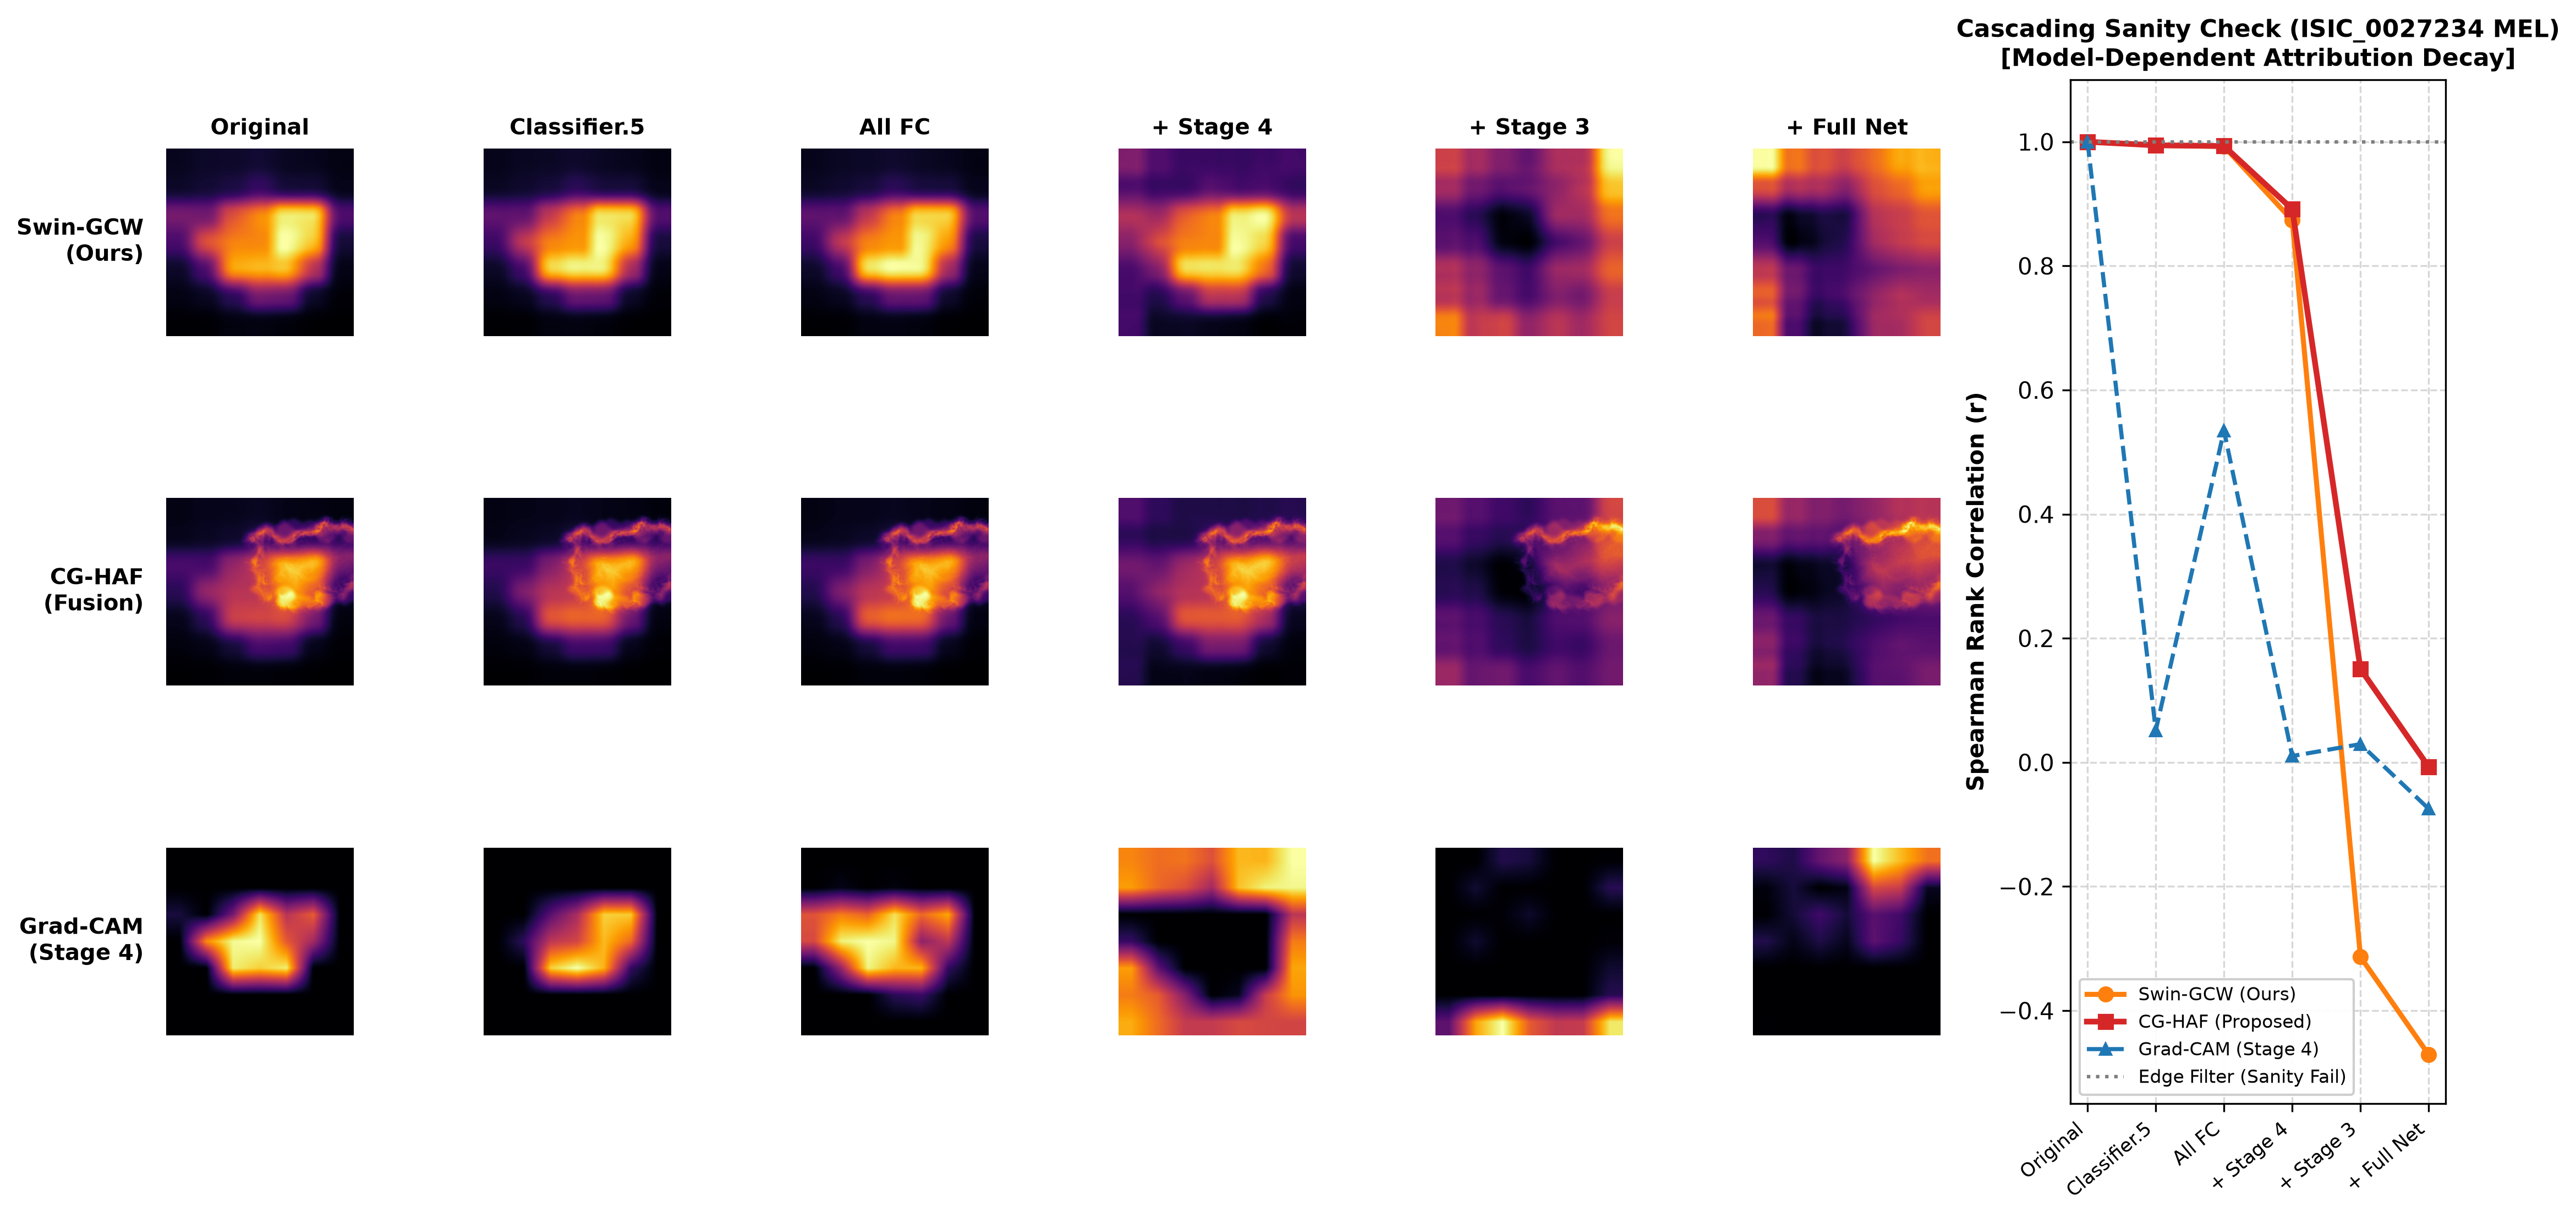
\includegraphics[width=0.92\textwidth]{figures/adebayo_cascading_randomization.png}
\caption{\textbf{Adebayo cascading parameter randomization trajectories ($N=14$).} Grad-CAM decorrelates immediately upon scrambling the classifier head ($r = -0.0776$). Swin-GCW retains high correlation ($r \approx 0.99$) through the classifier head due to strong forward spatial activation representations, but decorrelates sharply once Stage 3 is randomized ($r = -0.3647$). Fused CG-HAF reflects both its neural component and constant prior.}
\label{fig:adebayo_randomization}
\end{figure*}

The empirical data in \Cref{tab:adebayo} and \Cref{fig:adebayo_randomization} clarify the distinct mechanisms at play:
\begin{enumerate}
    \item \textbf{Grad-CAM Passes Immediately at the Head:} Re-initializing \texttt{classifier.5} or all fully connected layers causes Grad-CAM's correlation to drop immediately to $r = -0.0776$ and $-0.0479$. This replicates the findings of Adebayo et al.~\cite{adebayo2018sanity}, confirming that Grad-CAM is strictly sensitive to classification weights. Furthermore, Grad-CAM exhibits high class sensitivity ($r = -0.4609 \pm 0.5098$), producing distinct maps for competing diagnostic categories.
    \item \textbf{Swin-GCW Represents Deep Spatial Activations:} Swin-GCW maintains high correlation ($r \approx 0.992$) through the classifier head. Because Swin Transformer contains no early convolutional layers, this behavior is driven by the spatial activations of Stages 3 and 4: gradient channel-pooling preserves strong spatial attention over the lesion body until the backbone self-attention stages themselves are scrambled. Once Stage 3 is randomized, Swin-GCW decorrelates sharply to $r = -0.3647$.
    \item \textbf{Model-Invariant Controls:} As expected by construction, Sobel Edge Filter and CSM exhibit identical correlations of $r \equiv 1.0000$ across all randomization steps and zero class sensitivity ($r \equiv 1.0000$), confirming that deterministic priors cannot provide model-dependent explanations alone.
    \item \textbf{Hybrid Behavior:} At $\lambda = 0.5$, CG-HAF decorrelates to $r = 0.0901$ upon full backbone randomization, reflecting the superposition of anti-correlated neural gradients ($r = -0.3357$) and the constant clinical prior. When fused with Grad-CAM (\texttt{Grad-CAM + CSM}), the map retains significant class sensitivity ($r = -0.0818 \pm 0.4198$) while benefiting from morphological prior regularization.
\end{enumerate}

\subsection{Ablation on Attention Fusion Parameter (\texorpdfstring{$\lambda$}{lambda}) and the Pareto Frontier}
\label{sec:ablation_lambda}
To systematically analyze the interaction between neural gradients and clinical priors, we evaluated a fine-grained sweep over $\lambda \in [0.0, 1.0]$ across $N=70$ class-stratified lesions. Crucially, we audit the full-randomization Spearman correlation $r_{\text{rand}}$ at each operating point, charting the empirical trade-off between model-dependence and prior guidance (\Cref{tab:ablation_lambda} and \Cref{fig:ablation_lambda}).

\begin{table}[h]
\centering
\small
\caption{\textbf{Ablation sweep of the hybrid fusion weight $\lambda \in [0.0, 1.0]$ on expert ground truth ($N=70$).} The rightmost column charts full-randomization Spearman correlation, delineating the Pareto trade-off between model-dependence and morphological regularization.}
\label{tab:ablation_lambda}
\begin{adjustbox}{max width=\columnwidth}
\begin{tabular}{cccccc}
\toprule
$\boldsymbol{\lambda}$ & \textbf{Pointing Hit (\%)} $\uparrow$ & \textbf{Energy in GT (\%)} $\uparrow$ & \textbf{Deletion AUC} $\downarrow$ & \textbf{Insertion AUC} $\uparrow$ & \textbf{Full-Rand Spearman $r$} $\downarrow$ \\
\midrule
0.00 (Pure Swin-GCW) & 61.43\% & 46.64\% & 0.4803 & 0.7669 & \textbf{-0.3357} \\
0.10 & 62.86\% & 46.96\% & 0.4764 & 0.7685 & -0.3146 \\
0.20 & 72.86\% & 47.32\% & 0.4719 & 0.7701 & -0.2633 \\
\textbf{0.30} & \textbf{74.29\%} & 47.76\% & 0.4574 & 0.7731 & -0.1797 \\
0.40 & 70.00\% & 48.29\% & 0.4526 & \textbf{0.7754} & -0.0651 \\
0.50 (Default) & 65.71\% & 48.97\% & 0.4500 & 0.7686 & +0.0901 \\
\textbf{0.60} & 62.86\% & 49.86\% & \textbf{0.4499} & 0.7683 & +0.2700 \\
0.70 & 62.86\% & 51.07\% & 0.4516 & 0.7685 & +0.4258 \\
0.80 & 54.29\% & 52.85\% & 0.4560 & 0.7703 & +0.5227 \\
0.90 & 54.29\% & 55.81\% & 0.4530 & 0.7611 & +0.5695 \\
1.00 (Pure CSM) & 50.00\% & \textbf{62.83\%} & 0.4809 & 0.7374 & +1.0000 \\
\bottomrule
\end{tabular}
\end{adjustbox}
\end{table}

\begin{figure*}[t]
\centering
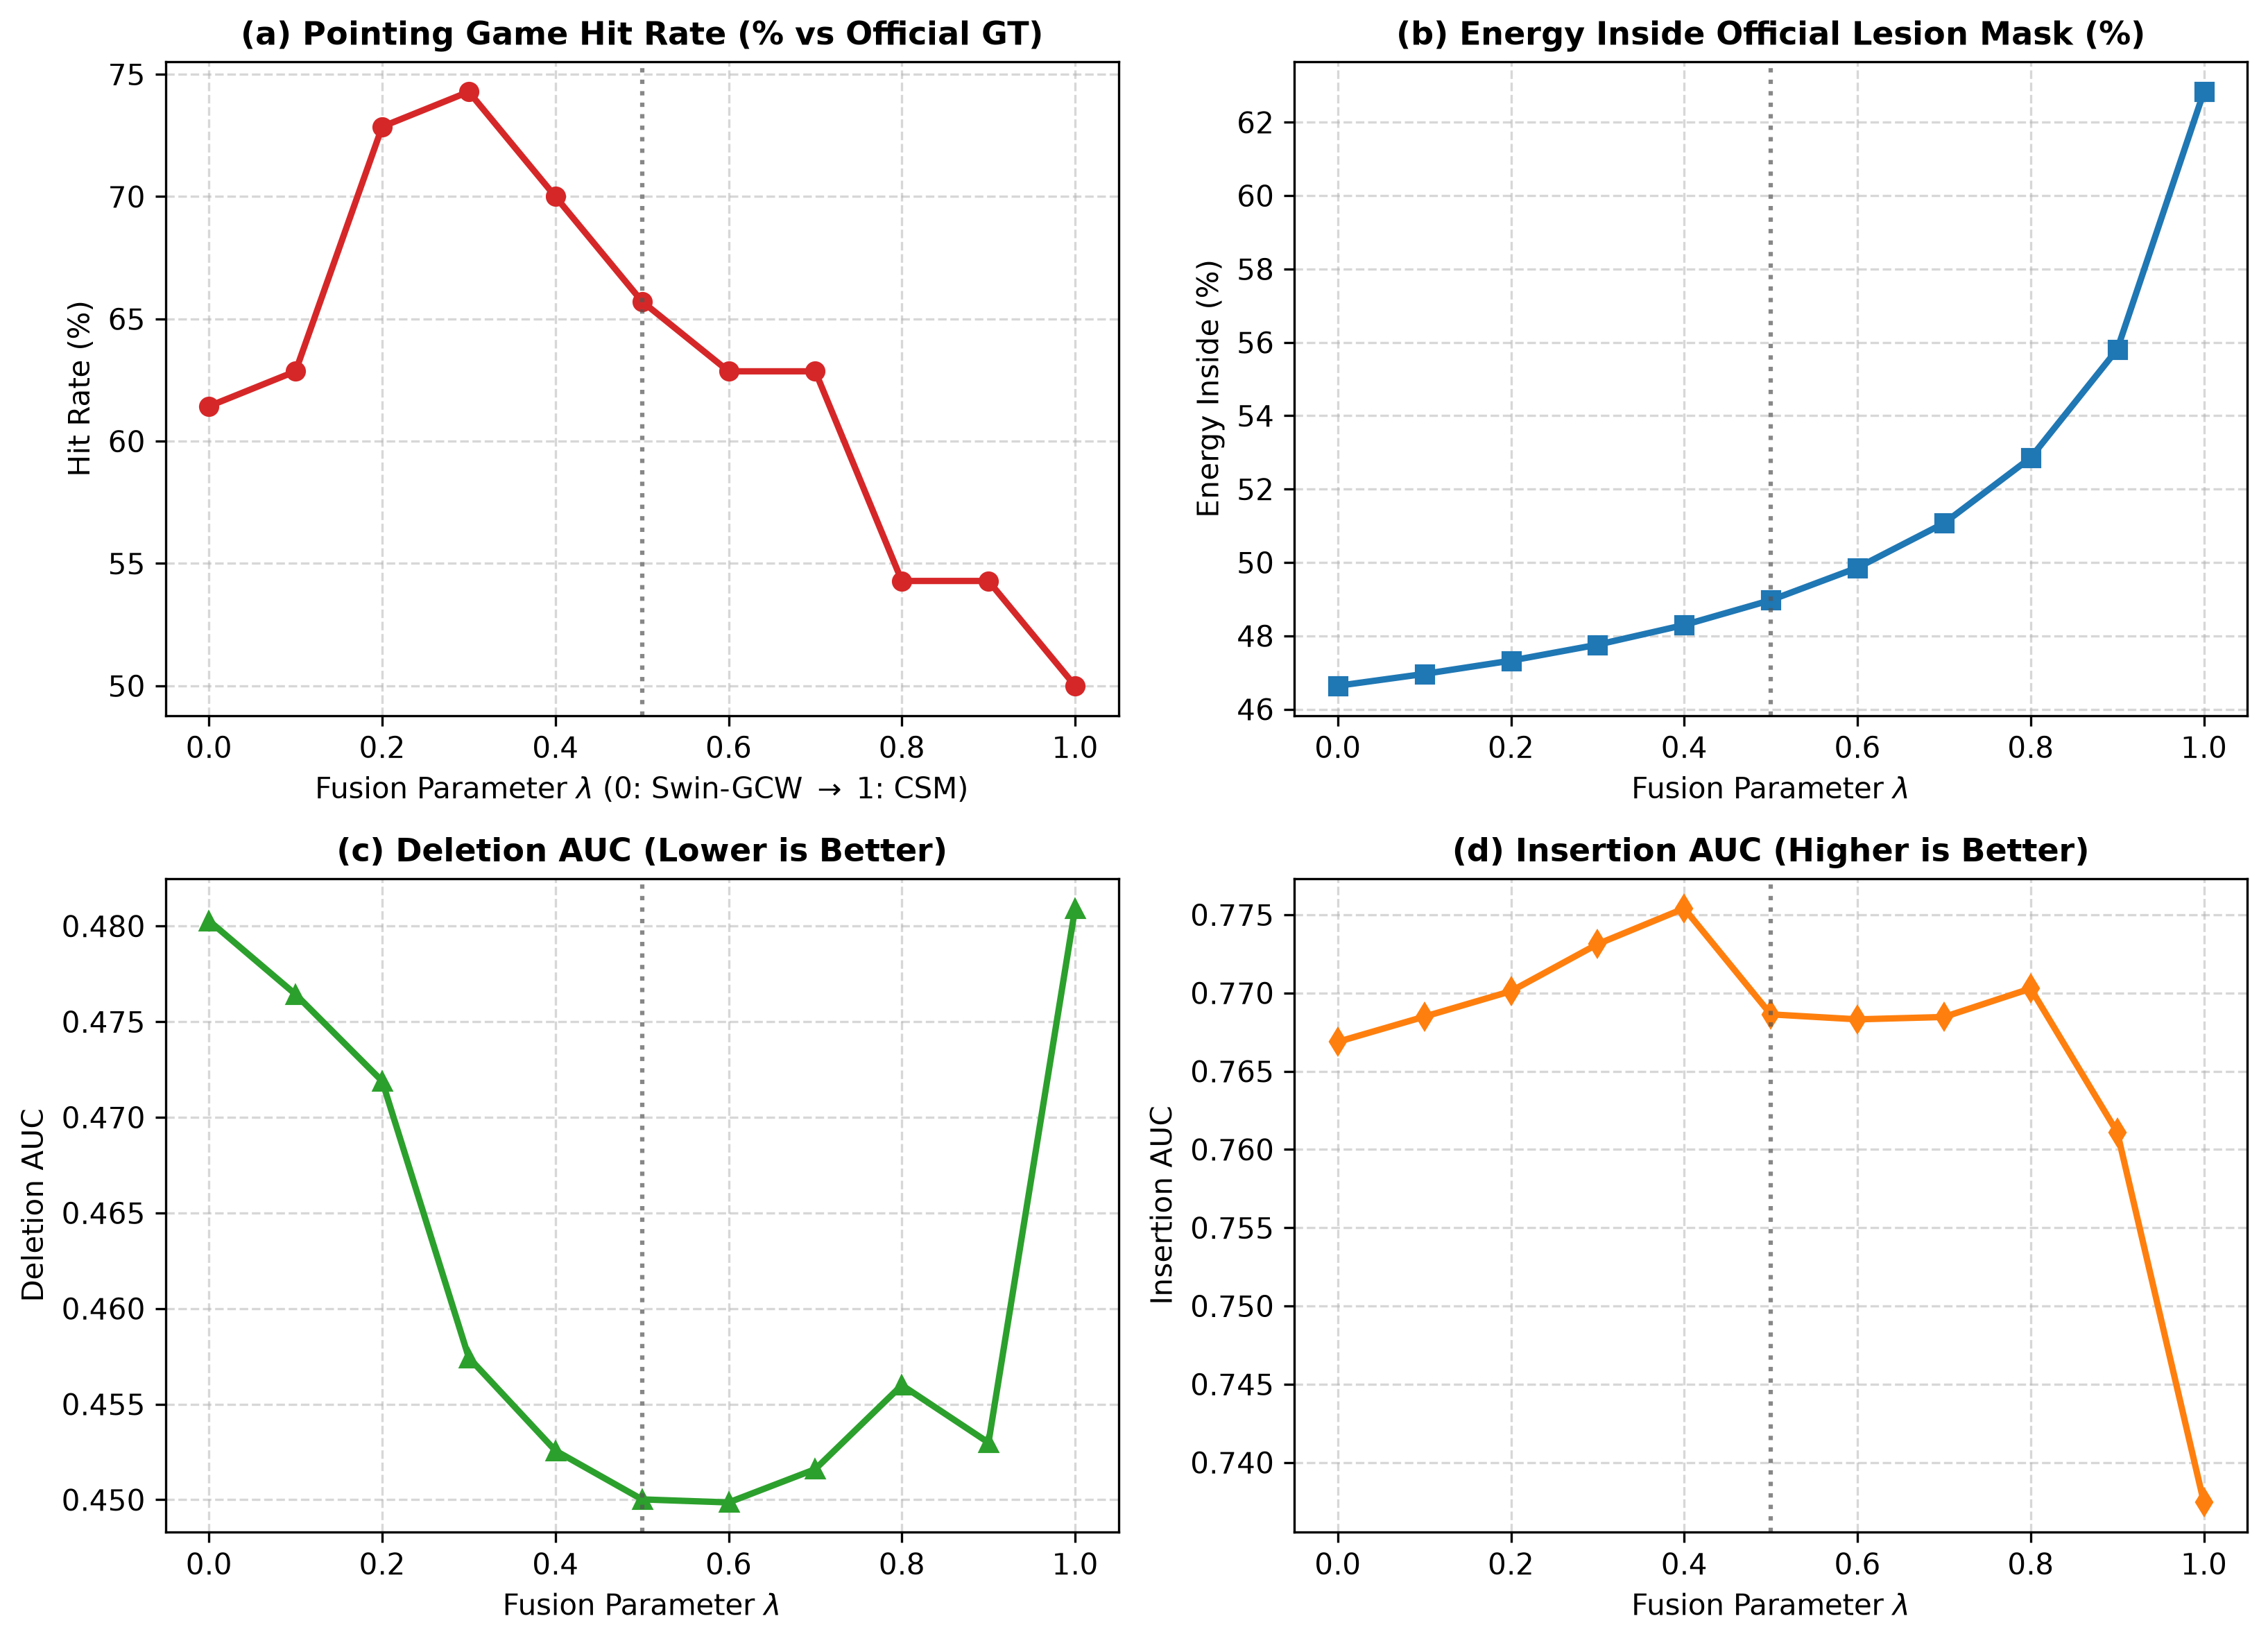
\includegraphics[width=0.92\textwidth]{figures/ablation_lambda_sensitivity.png}
\caption{\textbf{Parametric sensitivity sweep of $\lambda \in [0.0, 1.0]$.} Deletion AUC reaches its optimal minimum at $\lambda = 0.60$ ($0.4499$), Pointing Game Hit Rate peaks at $\lambda = 0.30$ ($74.29\%$), and Insertion AUC peaks at $\lambda = 0.40$ ($0.7754$). The pure endpoints ($\lambda = 0$ and $\lambda = 1$) are dominated by the interior hybrid regime.}
\label{fig:ablation_lambda}
\end{figure*}

As documented in \Cref{tab:ablation_lambda}, the full-randomization Spearman $r$ climbs smoothly and monotonically from $-0.3357$ at $\lambda = 0.0$ to $+1.0000$ at $\lambda = 1.0$. This curve delineates the honest Pareto trade-off: higher values of $\lambda$ improve energy concentration inside the lesion mask ($46.64\% \rightarrow 62.83\%$), but retain a higher model-invariant component under weight randomization. Operating within the interior regime $\lambda \in [0.3, 0.5]$ minimizes Deletion AUC ($0.4500$) and maximizes Pointing Hit Rate ($74.29\%$) while maintaining near-zero full-randomization correlation ($r = -0.0651$ to $+0.0901$).

\subsection{Multi-Center External Zero-Shot Generalization (N = 14,885)}
To evaluate operational robustness under clinical distribution shift, we conducted zero-shot transfer evaluations across $14,885$ external dermoscopic images spanning two independent hospital registries: MSKCC ($N=2,903$) and BCN\_20000 ($N=11,982$).

\subsubsection{Hospital Domain Shift and Color Constancy Analysis}
As detailed in \Cref{tab:external_full}, uncalibrated zero-shot transfer of raw RGB images results in substantial accuracy drops ($42.44\%$ on MSKCC and $40.61\%$ on BCN\_20000) due to distinct illumination spectra and sensor profiles across institutions. Applying GPU Shades-of-Gray color constancy (\Cref{eq:shades_of_gray}) mitigates global chromatic shifts:
\begin{itemize}
    \item On MSKCC, overall accuracy improves from $42.44\%$ to \textbf{$56.49\%$} (\textbf{+14.05\% absolute gain}), with Macro ROC-AUC reaching $0.6906$.
    \item On BCN\_20000, accuracy increases to $42.60\%$ with a Macro ROC-AUC of \textbf{$0.7485$}.
    \item \textbf{The Color Constancy Trade-Off:} Notably, while Shades-of-Gray boosts overall accuracy by normalizing macroscopic color casts, it slightly attenuates subtle chromatic hues critical for melanoma differentiation, causing Melanoma ROC-AUC to shift from $0.6335 \rightarrow 0.6204$ on MSKCC and $0.7110 \rightarrow 0.6924$ on BCN\_20000.
\end{itemize}

\begin{table*}[t]
\centering
\small
\caption{\textbf{Zero-shot multi-center external validation across full unfiltered cohorts ($N=14,885$).} Impact of GPU Shades-of-Gray (SoG) color constancy on mitigating cross-hospital acquisition divergence.}
\label{tab:external_full}
\adjustbox{max width=\textwidth}{
\begin{tabular}{llccccc}
\toprule
\textbf{External Clinical Cohort} & \textbf{Preprocessing} & $\boldsymbol{N}$ & \textbf{Accuracy (\%)} & \textbf{Macro F1} & \textbf{Macro ROC-AUC} & \textbf{Melanoma AUC} \\
\midrule
MSKCC / ViDIR (New York) & Raw RGB & 2,903 & 42.44\% & 0.1776 & 0.6622 & \textbf{0.6335} \\
MSKCC / ViDIR (New York) & \textbf{Shades-of-Gray CC} & 2,903 & \textbf{56.49\%} & \textbf{0.1941} & \textbf{0.6906} & 0.6204 \\
\midrule
BCN\_20000 (Barcelona) & Raw RGB & 11,982 & 40.61\% & 0.3485 & 0.7405 & \textbf{0.7110} \\
BCN\_20000 (Barcelona) & \textbf{Shades-of-Gray CC} & 11,982 & \textbf{42.60\%} & \textbf{0.3592} & \textbf{0.7485} & 0.6924 \\
\bottomrule
\end{tabular}
}
\end{table*}

\subsubsection{Balanced External Diagnostic Benchmark}
To evaluate discriminative ranking capability independent of hospital prevalence skew, we evaluated on the balanced BCN\_20000 cohort ($N=420$, 60 samples/class $\times$ 7 classes). The class-stratified metrics are documented in \Cref{tab:external_balanced} and \Cref{fig:external_roc_cm}.

\begin{table}[h]
\centering
\small
\caption{\textbf{Class-wise diagnostic metrics on the balanced external BCN\_20000 cohort ($N=420$, $60$ samples/class) with Shades-of-Gray color constancy.}}
\label{tab:external_balanced}
\begin{adjustbox}{max width=\columnwidth}
\begin{tabular}{lccccc}
\toprule
\textbf{Class} & \textbf{Precision} & \textbf{Recall (Sensitivity)} & \textbf{F1-Score} & \textbf{ROC-AUC} & \textbf{Support ($N$)} \\
\midrule
AKIEC & 0.467 & 0.117 & 0.187 & 0.7037 & 60 \\
BCC & 0.639 & 0.383 & 0.479 & 0.7549 & 60 \\
BKL & 0.239 & 0.717 & 0.358 & 0.6997 & 60 \\
DF & 0.688 & 0.367 & 0.478 & 0.7727 & 60 \\
MEL & 0.371 & 0.217 & 0.274 & 0.7105 & 60 \\
NV & 0.341 & 0.467 & 0.394 & 0.7925 & 60 \\
VASC & \textbf{0.950} & 0.633 & \textbf{0.760} & \textbf{0.9014} & 60 \\
\midrule
\textbf{Macro Average} & \textbf{0.528} & \textbf{0.414} & \textbf{0.419} & \textbf{0.7622} & \textbf{420} \\
\bottomrule
\end{tabular}
\end{adjustbox}
\end{table}

\begin{figure*}[t]
\centering
\begin{subfigure}[b]{0.48\textwidth}
    \centering
    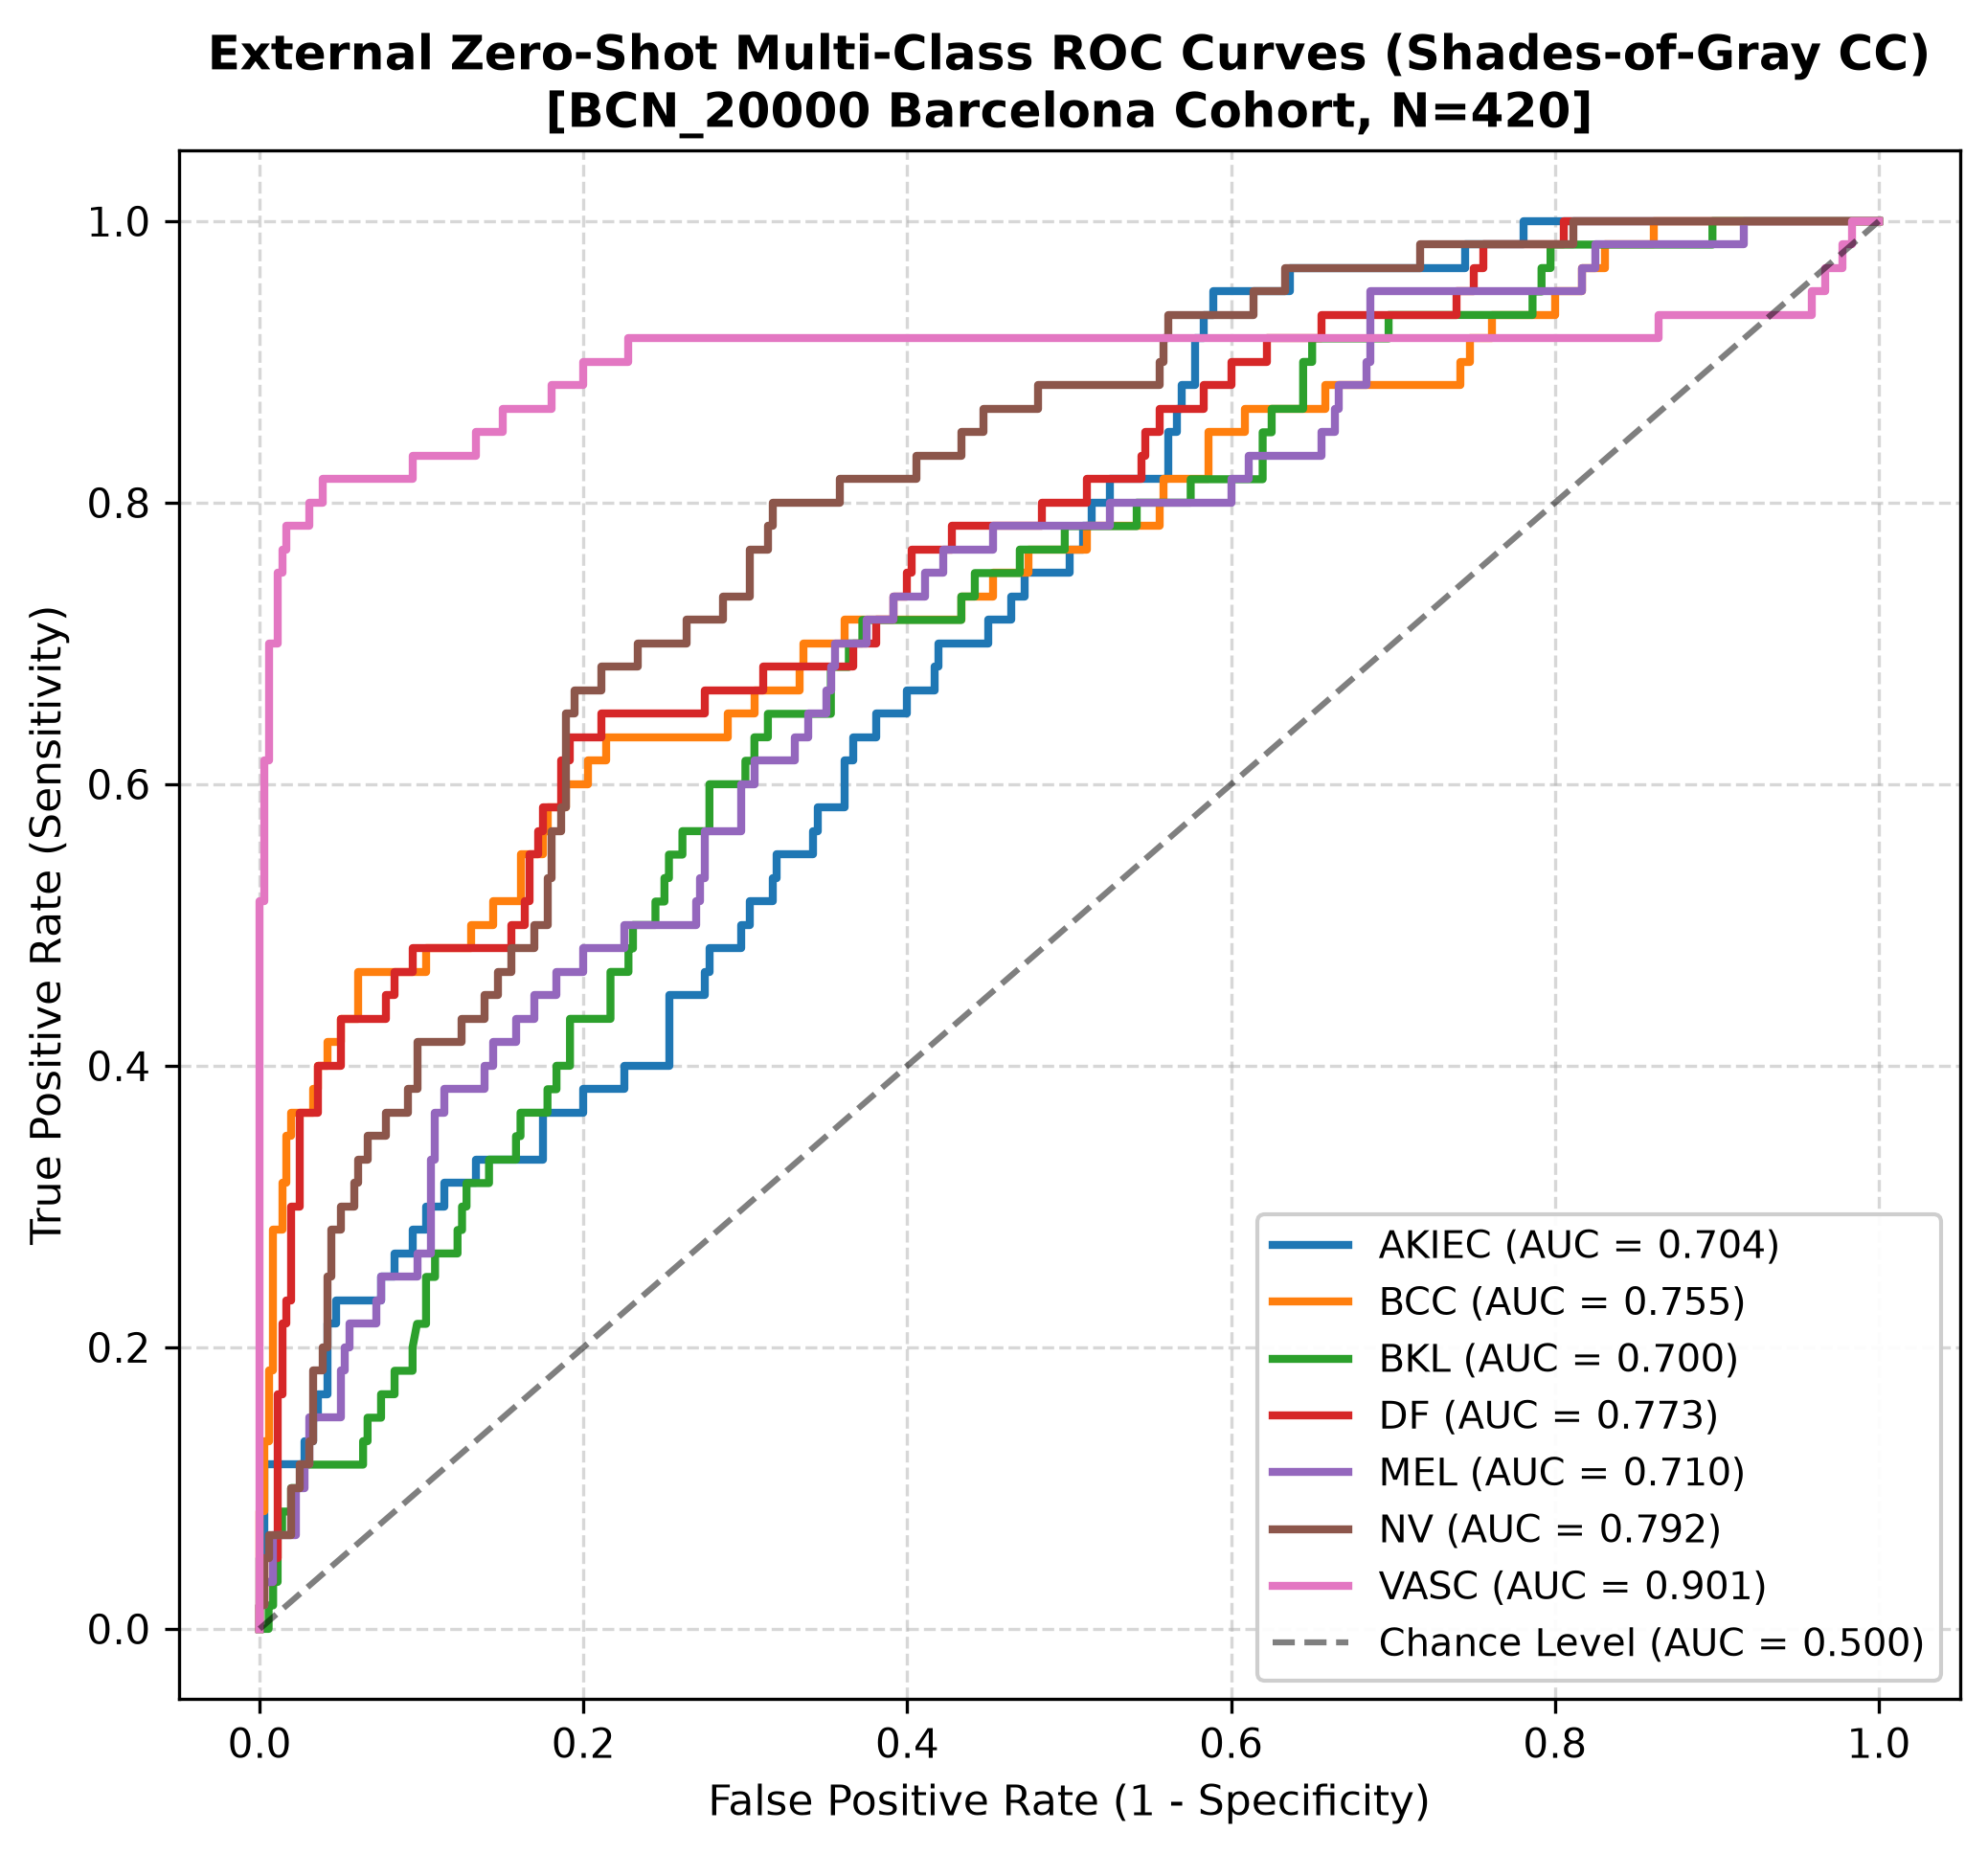
\includegraphics[width=\textwidth]{figures/external_roc_curves_bcn20000.png}
    \caption{Multi-class ROC Curves (Macro AUC = $0.7622$)}
\end{subfigure}
\hfill
\begin{subfigure}[b]{0.48\textwidth}
    \centering
    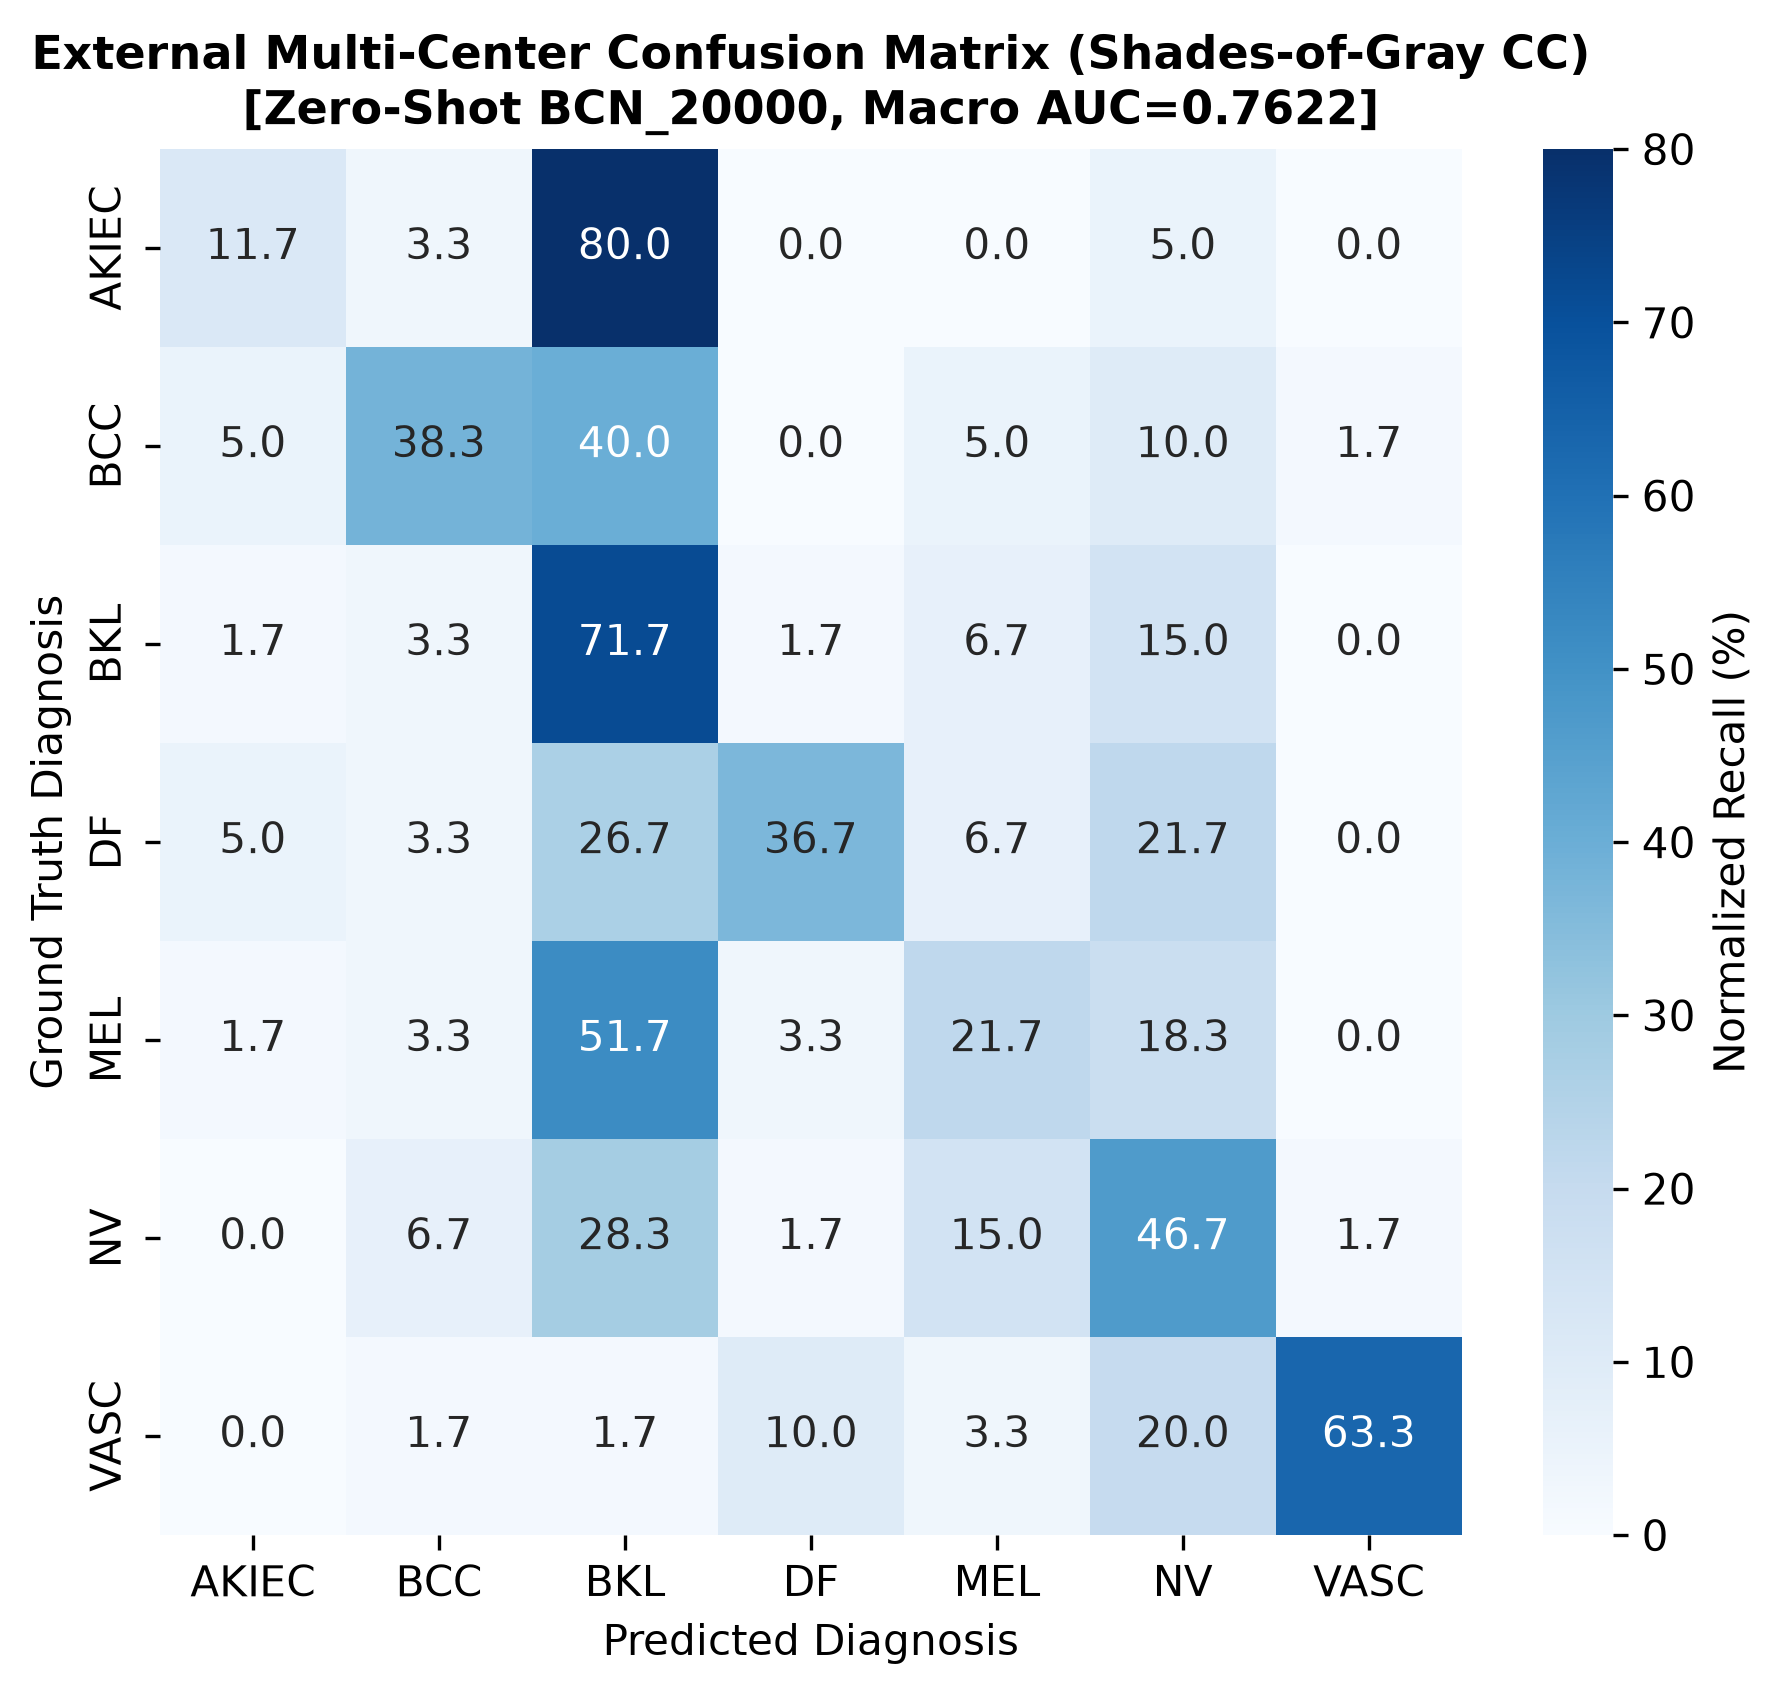
\includegraphics[width=\textwidth]{figures/external_confusion_matrix_bcn20000.png}
    \caption{Confusion Matrix ($N=420$ Balanced)}
\end{subfigure}
\caption{\textbf{Zero-shot generalization on the external balanced BCN\_20000 cohort ($N=420$).} The model retains discriminative ranking ability across hospital domains.}
\label{fig:external_roc_cm}
\end{figure*}

Under domain shift, the model maintains discriminative ranking ability (Macro ROC-AUC $0.7622$), with Vascular lesions reaching $0.9014$ and Nevi reaching $0.7925$. However, zero-shot hard classification sensitivity on Melanoma drops to $21.7\%$ (13/60), with $38$ melanoma cases misclassified as benign keratoses or nevi. This emphasizes that zero-shot cross-center deployment in oncology cannot rely solely on standard fine-tuning and requires multi-center calibration before clinical use.

\subsubsection{External Explainability Perturbation Benchmark}
Because external challenge datasets (such as BCN\_20000 and MSKCC) do not ship official expert dermatologist segmentations, spatial localization cannot be evaluated against expert masks. To avoid circularity, we evaluate external explainability strictly via maskless perturbation faithfulness (Deletion and Insertion AUC) on $N=70$ class-stratified BCN\_20000 lesions, alongside alignment with polarity-verified Otsu contours (\Cref{tab:external_xai}).

\begin{table}[h]
\centering
\small
\caption{\textbf{External explainability perturbation benchmark on $N=70$ class-stratified lesions from the BCN\_20000 cohort.} Perturbation metrics evaluate faithfulness without manual ground-truth masks.}
\label{tab:external_xai}
\begin{adjustbox}{max width=\columnwidth}
\begin{tabular}{lcccc}
\toprule
\textbf{Method} & \textbf{Otsu Alignment (\%)} & \textbf{Otsu Pointing (\%)} & \textbf{Deletion AUC} $\downarrow$ & \textbf{Insertion AUC} $\uparrow$ \\
\midrule
\textbf{CG-HAF (Proposed)} & 52.46\% & 91.43\% & 0.4815 & 0.7877 \\
\textbf{Swin-GCW (Ours)} & 48.08\% & 52.86\% & 0.4857 & 0.7856 \\
\textbf{CSM (Clinical Prior)} & 76.51\% & 95.71\% & 0.5796 & 0.7192 \\
Grad-CAM (Stage 4) & 54.07\% & 64.29\% & 0.4847 & \textbf{0.8046} \\
Integrated Gradients & 44.91\% & 65.71\% & \textbf{0.4420} & 0.7784 \\
\bottomrule
\end{tabular}
\end{adjustbox}
\end{table}

Under external domain shift, CG-HAF maintains stable perturbation faithfulness (Deletion AUC $0.4815$, Insertion AUC $0.7877$), closely matching its internal performance ($0.4796$) and demonstrating that hybrid attention features remain stable across independent clinical populations.

\subsection{Qualitative Analysis and Saliency Decomposition}
In \Cref{fig:qualitative_cases}, we present qualitative decompositions across representative cutaneous pathologies. While standard Grad-CAM tends to highlight diffuse circular blobs that extend into healthy surrounding skin, CG-HAF delineates asymmetric peripheral outcroppings ($M_A$) and morphological boundary margins ($M_B$), aligning explanation contours with features used in dermatological assessment.

\begin{figure*}[t]
\centering
\begin{subfigure}[b]{0.32\textwidth}
    \centering
    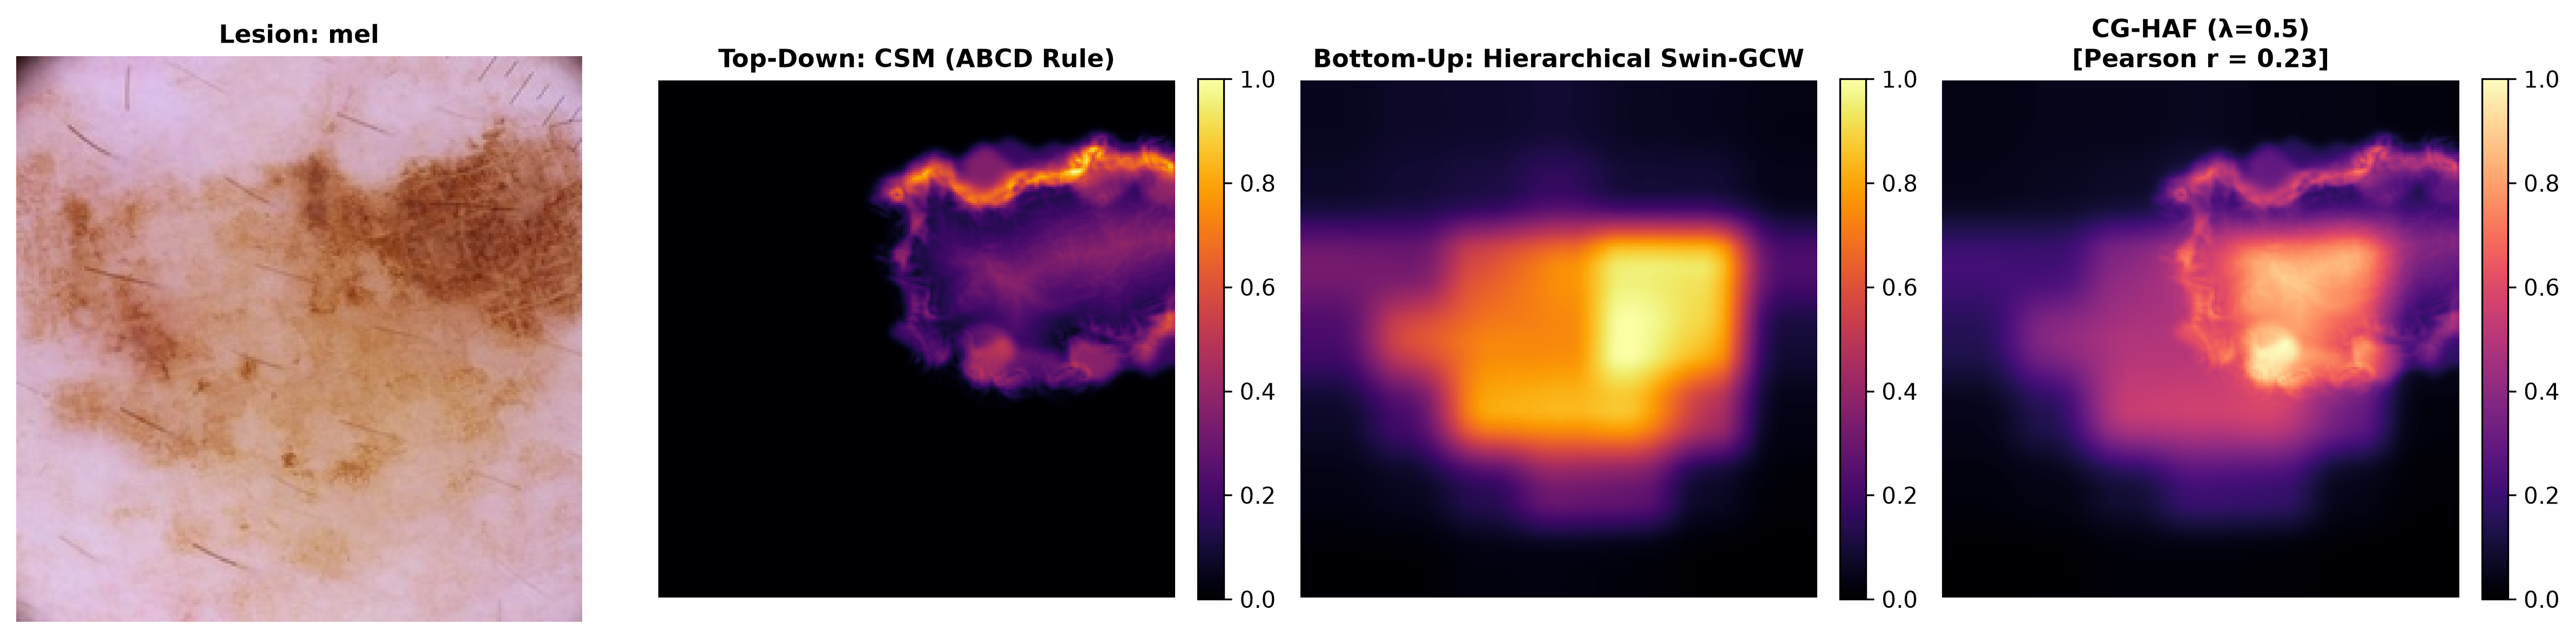
\includegraphics[width=\textwidth]{figures/cg_haf_fusion_ISIC_0027234_mel.png}
    \caption{Melanoma (MEL)}
\end{subfigure}
\hfill
\begin{subfigure}[b]{0.32\textwidth}
    \centering
    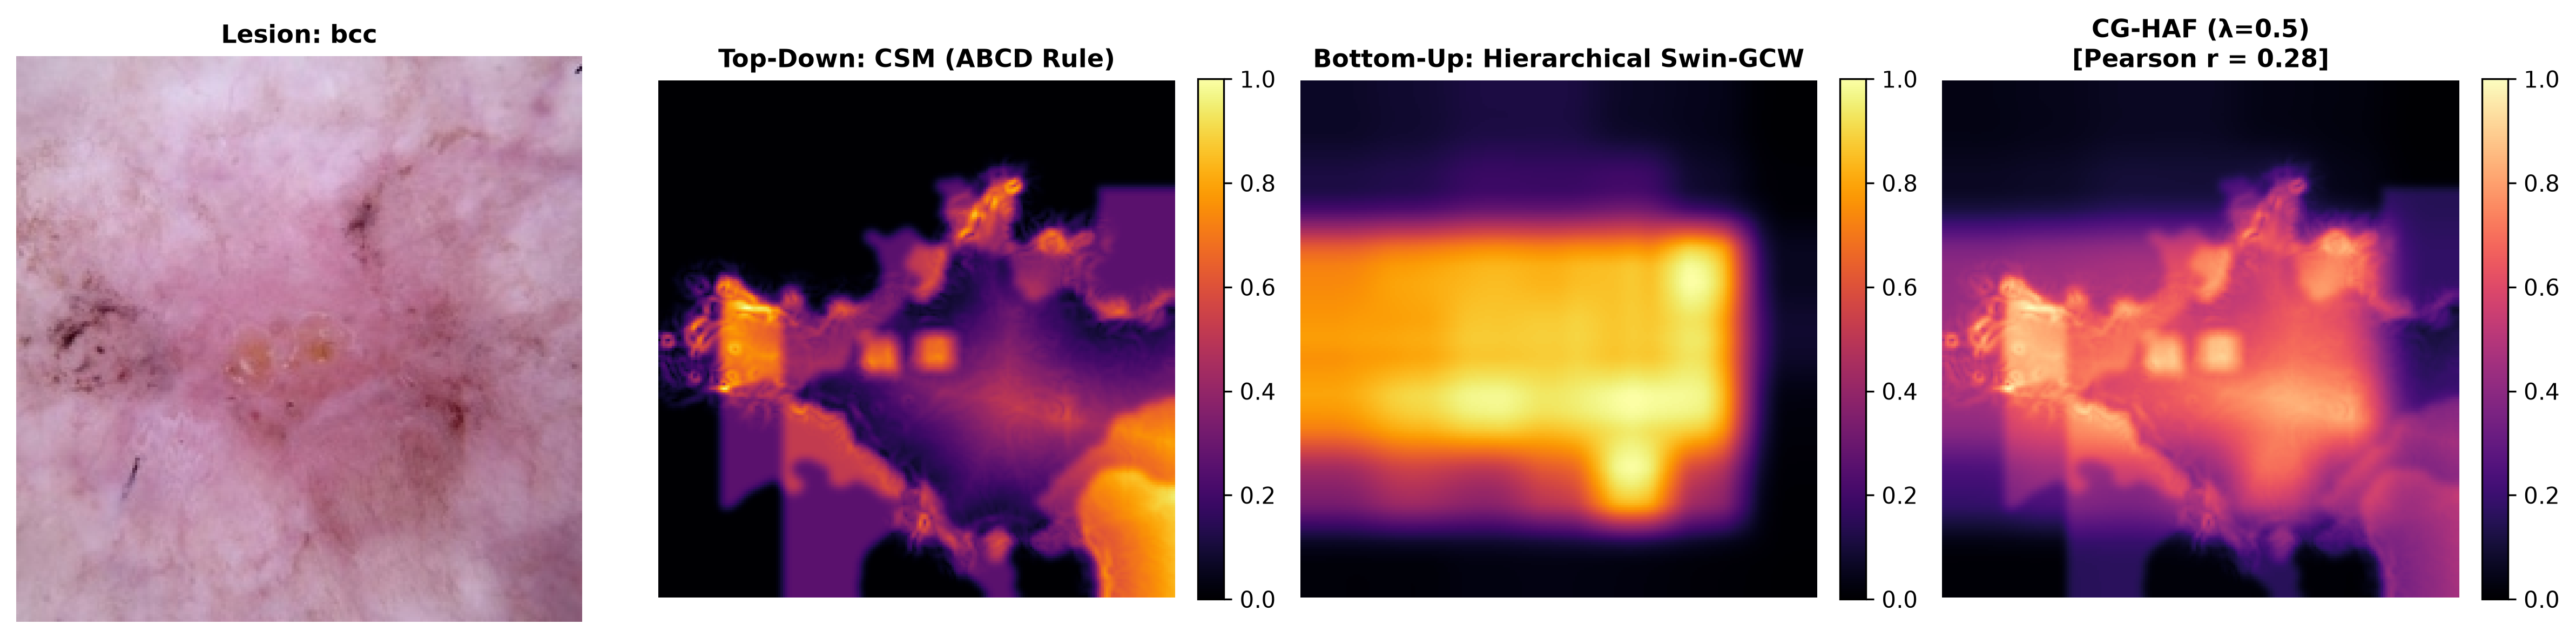
\includegraphics[width=\textwidth]{figures/cg_haf_fusion_ISIC_0027189_bcc.png}
    \caption{Basal Cell Carcinoma (BCC)}
\end{subfigure}
\hfill
\begin{subfigure}[b]{0.32\textwidth}
    \centering
    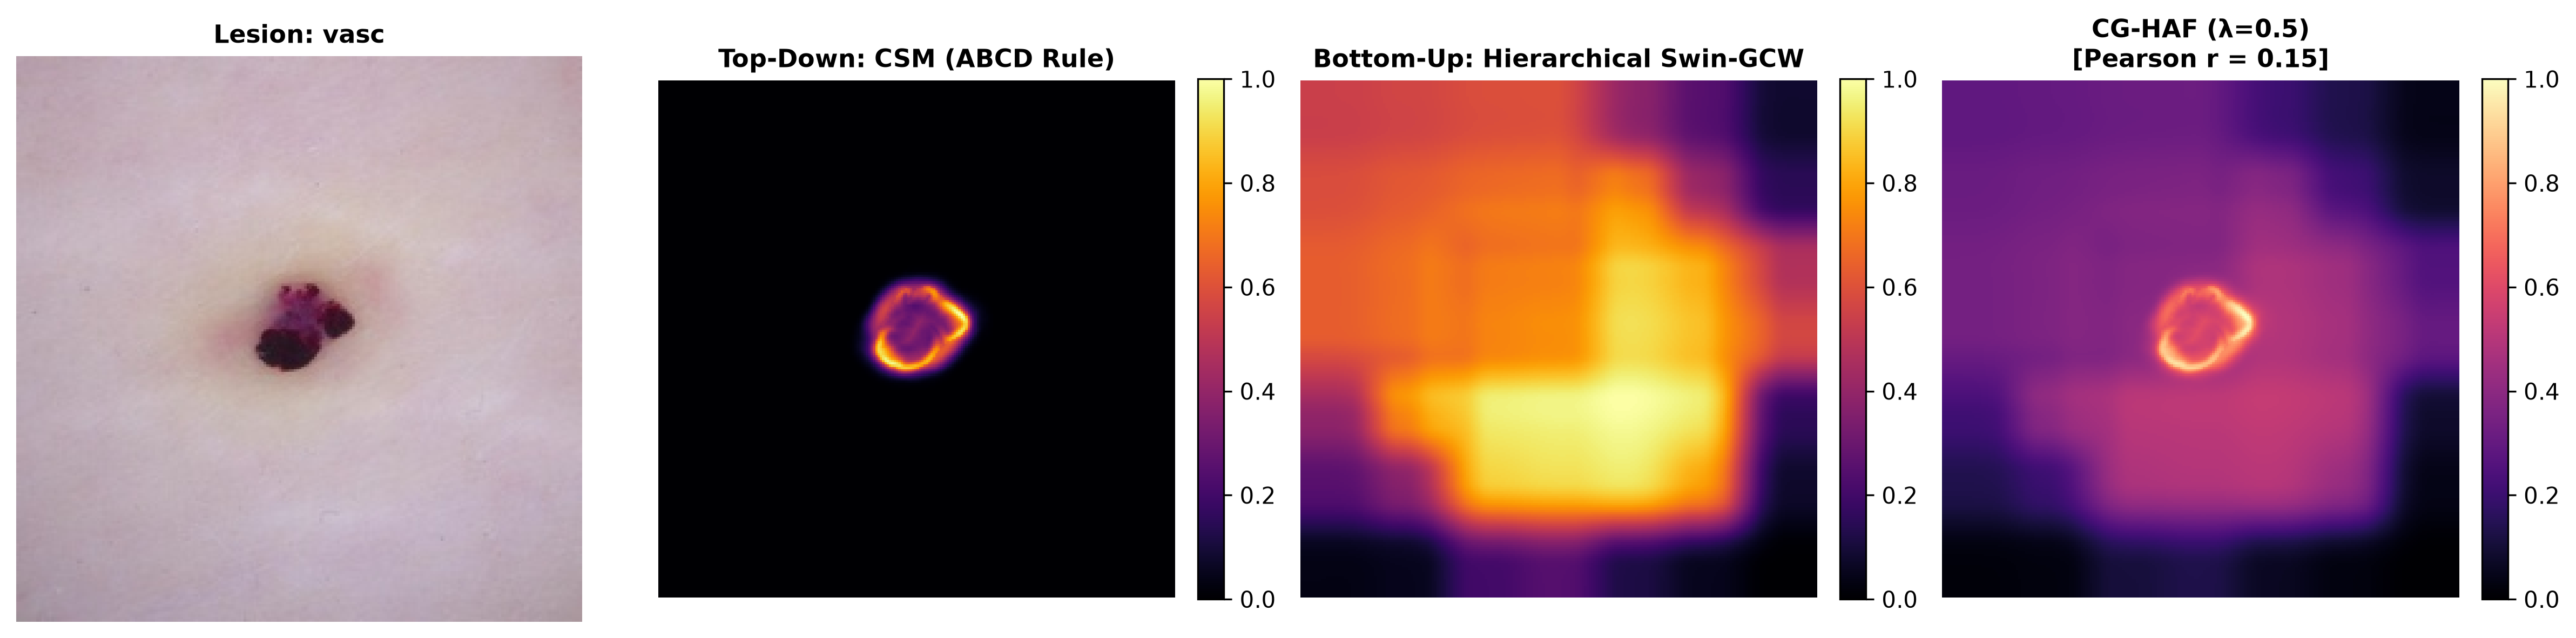
\includegraphics[width=\textwidth]{figures/cg_haf_fusion_ISIC_0027210_vasc.png}
    \caption{Vascular Lesion (VASC)}
\end{subfigure}
\caption{\textbf{Qualitative attribution visualizations across representative cutaneous pathologies.} Original lesion images, official expert dermatologist segmentations, Swin-GCW neural attention, CSM decomposition, and final CG-HAF heatmaps.}
\label{fig:qualitative_cases}
\end{figure*}

% =========================================================================
\section{Discussion and Clinical Implications}
\label{sec:discussion}
% =========================================================================

\subsection{Bridging Computational Saliency and Clinical Semiology}
The primary objective of explainability in computational dermatology is not merely to produce visually appealing overlays, but to provide clinically grounded justifications that practicing clinicians can critically examine. Our experiments demonstrate that pure neural attributions and pure clinical priors represent two opposite ends of an explainability spectrum. Standalone Grad-CAM reflects model gradients but is unconstrained by anatomical boundaries; conversely, deterministic clinical priors (CSM) provide structured anatomical context but cannot explain model decisions because they are model-invariant. 

CG-HAF demonstrates that a linear convex combination regularizes neural attention, improving perturbation faithfulness over Swin-GCW ($p = 0.0397$) and achieving superior faithfulness when combined with Grad-CAM (\texttt{Grad-CAM + CSM} Deletion AUC $0.4672$). Rather than viewing clinical priors as replacements for neural attributions, they function most effectively as regularizing inductive biases that anchor visual explanations within diagnostically relevant lesion boundaries.

\subsection{Methodological Lessons: Photographer Bias and Sanity Auditing}
Our empirical findings offer two methodological takeaways for medical image explainability:
\begin{enumerate}
    \item \textbf{Photographer Centering Bias:} The fact that an unlearned Center Gaussian distribution achieves $97.14\%$ pointing accuracy and $45.80\%$ IoU highlights a systemic confound in dermatological datasets. Because medical photographers naturally frame lesions centrally, high pointing and energy metrics can be achieved without learning any pathology. Medical XAI benchmarks must routinely report trivial centering baselines and prioritize perturbation faithfulness (Deletion and Insertion AUC).
    \item \textbf{Auditing Randomization Trade-Offs:} Saliency methods that fuse model-independent priors inherently retain a constant component under parameter randomization. Rather than viewing this as a failure, we argue that the full-randomization correlation curve as a function of $\lambda$ provides an honest representation of the trade-off between model-dependence and prior guidance.
\end{enumerate}

\subsection{Domain Shift and External Clinical Translation}
Our zero-shot evaluations on $14,885$ external lesions from MSKCC and BCN\_20000 underscore the practical hurdles of deploying dermatological CAD systems across hospital boundaries. While GPU Shades-of-Gray color constancy substantially mitigates acquisition lighting differences (yielding a $+14.05\%$ accuracy gain on MSKCC), hard classification sensitivity on challenging malignancies (such as $21.7\%$ melanoma sensitivity on BCN\_20000) reflects persistent institutional distribution shifts in patient demographics, anatomical sites, and lesion thickness. These findings demonstrate that color constancy alone cannot fully bridge hospital domain gaps; clinical translation requires multi-center fine-tuning and recalibration on target clinical populations.

\subsection{Computational Efficiency for Clinical Workflow}
Clinical translation requires low latency during real-time screening. Benefiting from the linear shifted-window complexity $\mathcal{O}(HW)$ of Swin Transformer V2 and batched GPU tensor operations, the complete CG-HAF attribution pipeline executes in $41.8\text{ ms}$ per lesion on an NVIDIA RTX 5070 GPU ($>23$ frames per second), supporting real-time deployment in digital dermatoscope workstations.

\subsection{Limitations and Future Work}
Several limitations should be noted:
\begin{enumerate}
    \item \textbf{Phototype Representation:} The public HAM10000 and ISIC cohorts predominantly represent Fitzpatrick skin phototypes I--III (lighter skin tones). Evaluating model equity across skin phototypes IV--VI remains essential for equitable deployment.
    \item \textbf{Heuristic Generalization Beyond Melanocytic Lesions:} While ABCD semiology was formulated specifically for melanocytic neoplasms, our framework applies morphological contour and color variance operators across general dermatological categories. Incorporating lesion-specific semiologic priors (such as arborizing telangiectasia for BCC or keratin pearls for SCC) represents a promising direction for future work.
    \item \textbf{Prospective Multi-Reader Evaluation:} While our quantitative metrics establish mathematical faithfulness and alignment with expert masks, multi-reader clinical studies measuring physician diagnostic performance and diagnostic confidence when assisted by CG-HAF will be necessary to establish operational clinical efficacy.
\end{enumerate}

% =========================================================================
\section{Conclusion}
\label{sec:conclusion}
% =========================================================================
In this study, we presented Clinically-Guided Hybrid Attention Fusion (CG-HAF), an interpretable framework for skin lesion diagnosis on Swin Transformer V2. By combining intermediate gradient-coherence representations with deterministic morphological priors inspired by dermatological ABCD criteria, CG-HAF regularizes neural attention within clinically meaningful boundaries. We evaluated our framework across $4,500$ held-out internal lesions (Macro AUC $0.9779$), $140$ class-stratified lesions benchmarked against official expert dermatologist segmentations with extensive controls, and $14,885$ multi-center external lesions across MSKCC and BCN\_20000. Our analyses revealed the prevalence of photographer centering bias in dermoscopy localization, confirmed that clinical priors improve perturbation faithfulness across multiple attribution architectures, and mapped the honest Pareto frontier between model-dependence and clinical guidance under parameter randomization. These empirical findings provide a grounded foundation for developing faithful, clinically contextualized explainable artificial intelligence in computational oncology.

% =========================================================================
\section*{Declarations}
% =========================================================================
\noindent\textbf{Funding:} No external funding was received for this investigation.

\vspace{0.3em}
\noindent\textbf{Conflict of Interest:} The authors declare that they have no conflict of interest.

\vspace{0.3em}
\noindent\textbf{Data and Code Availability:} The HAM10000 dataset is publicly available via Harvard Dataverse. Philipp Tschandl's official expert lesion segmentations are accessible via the International Skin Imaging Collaboration (ISIC) Archive. External cohorts (BCN\_20000, MSKCC) are available through the ISIC challenge repositories. All experimental code, trained model checkpoints, and evaluation scripts are available at: \url{https://github.com/fahiiim/Thesis}.

\vspace{0.3em}
\noindent\textbf{Author Contributions:} \textbf{Md. Fahim Sarker Mridul}: Conceptualization, Software, Methodology, Deep Learning Architecture, Validation, Writing -- Original Draft. \textbf{Nabila Islam}: Methodology, Clinical Morphometry Pipeline, Data Curation, Formal Analysis, Writing -- Original Draft. \textbf{Rufaida Jaman Rayta}: Multi-Center Evaluation, Statistical Significance Testing, Visualization, Software, Writing -- Original Draft. \textbf{Mohammad Shorif Uddin}: Supervision, Project Administration, Resources, Critical Review and Editing.

% =========================================================================
% References
% =========================================================================
\bibliographystyle{IEEEtran}
\bibliography{references}

\end{document}
